\section{Adding Time Coherence}
\label[section]{sec:tcalg}
This section will be about how we translated the definition from \Cref{sec:tcdef} into a functional component for our algorithm.
We use the aforementioned energy measure to induce a process we refer to as \textit{coaxing},
as we are applying continued pressure to streamlines, moving them in the direction of their former footprints.

A second addition we call \textit{shattering} will be introduced as well,
where streamlines are split into smaller segments (\textit{fragments}) 
to be used as the starting layout for the next time step.
This can increase coherence as well by seeding streamlines at the same place,
and works especially well in combination with coaxing.

\subsection{Coaxing}
Since most of the algorithm's optimization is centered around the comparison
with an energy level before and after an action was taken,
modifying the energy function provides good leverage regarding how streamlines are placed. 
In order to make the algorithm favor previous streamline positions,
we therefore rewrite the previous energy function $E$ as the linear
interpolation between $E_s$ and $E_t$. This gives us good control over how much time coherence we apply, as choosing too much will cause a degradation in image quality.
Given the previous frame's low-pass image generated using the time kernel $L_t\ast I_0$ and the current image as $L_t\ast I_1$, we use:
\begin{equation*}
    \begin{split}
        E(I_0, I_1) &= \alpha E_s(I)+(1-\alpha)E_t(I_0, I_1)\\
        E_s(I_1)      &= \int_x\int_y\left[(L_s\ast I_1)(x,y)-t\right]^2\,\text{d}x\,\text{d}y\\
        E_t(I_0, I_1)  &= \int_x\int_y\left[(L_t\ast I_0)(x,y)-(L_t\ast I_1)(x,y)\right]^2\,\text{d}x\,\text{d}y
    \end{split}
\end{equation*}
We have found values for $\alpha$ in the range $[0.4, 0.8]$ to be effective.
Choosing a higher value causes very few streamlines to be drawn,
and only yields sporadic segments due to the inhibitory effect on the lengthen and
join operations when leaving the previous streamline's footprint.
This gets exacerbated by the gaps between the fragments being cemented in the new $L_t\ast I$,
not allowing them to reconnect in subsequent frames.

\begin{figure}[t]
    \centering
    \begin{subfigure}{.24\textwidth}
        \centering
        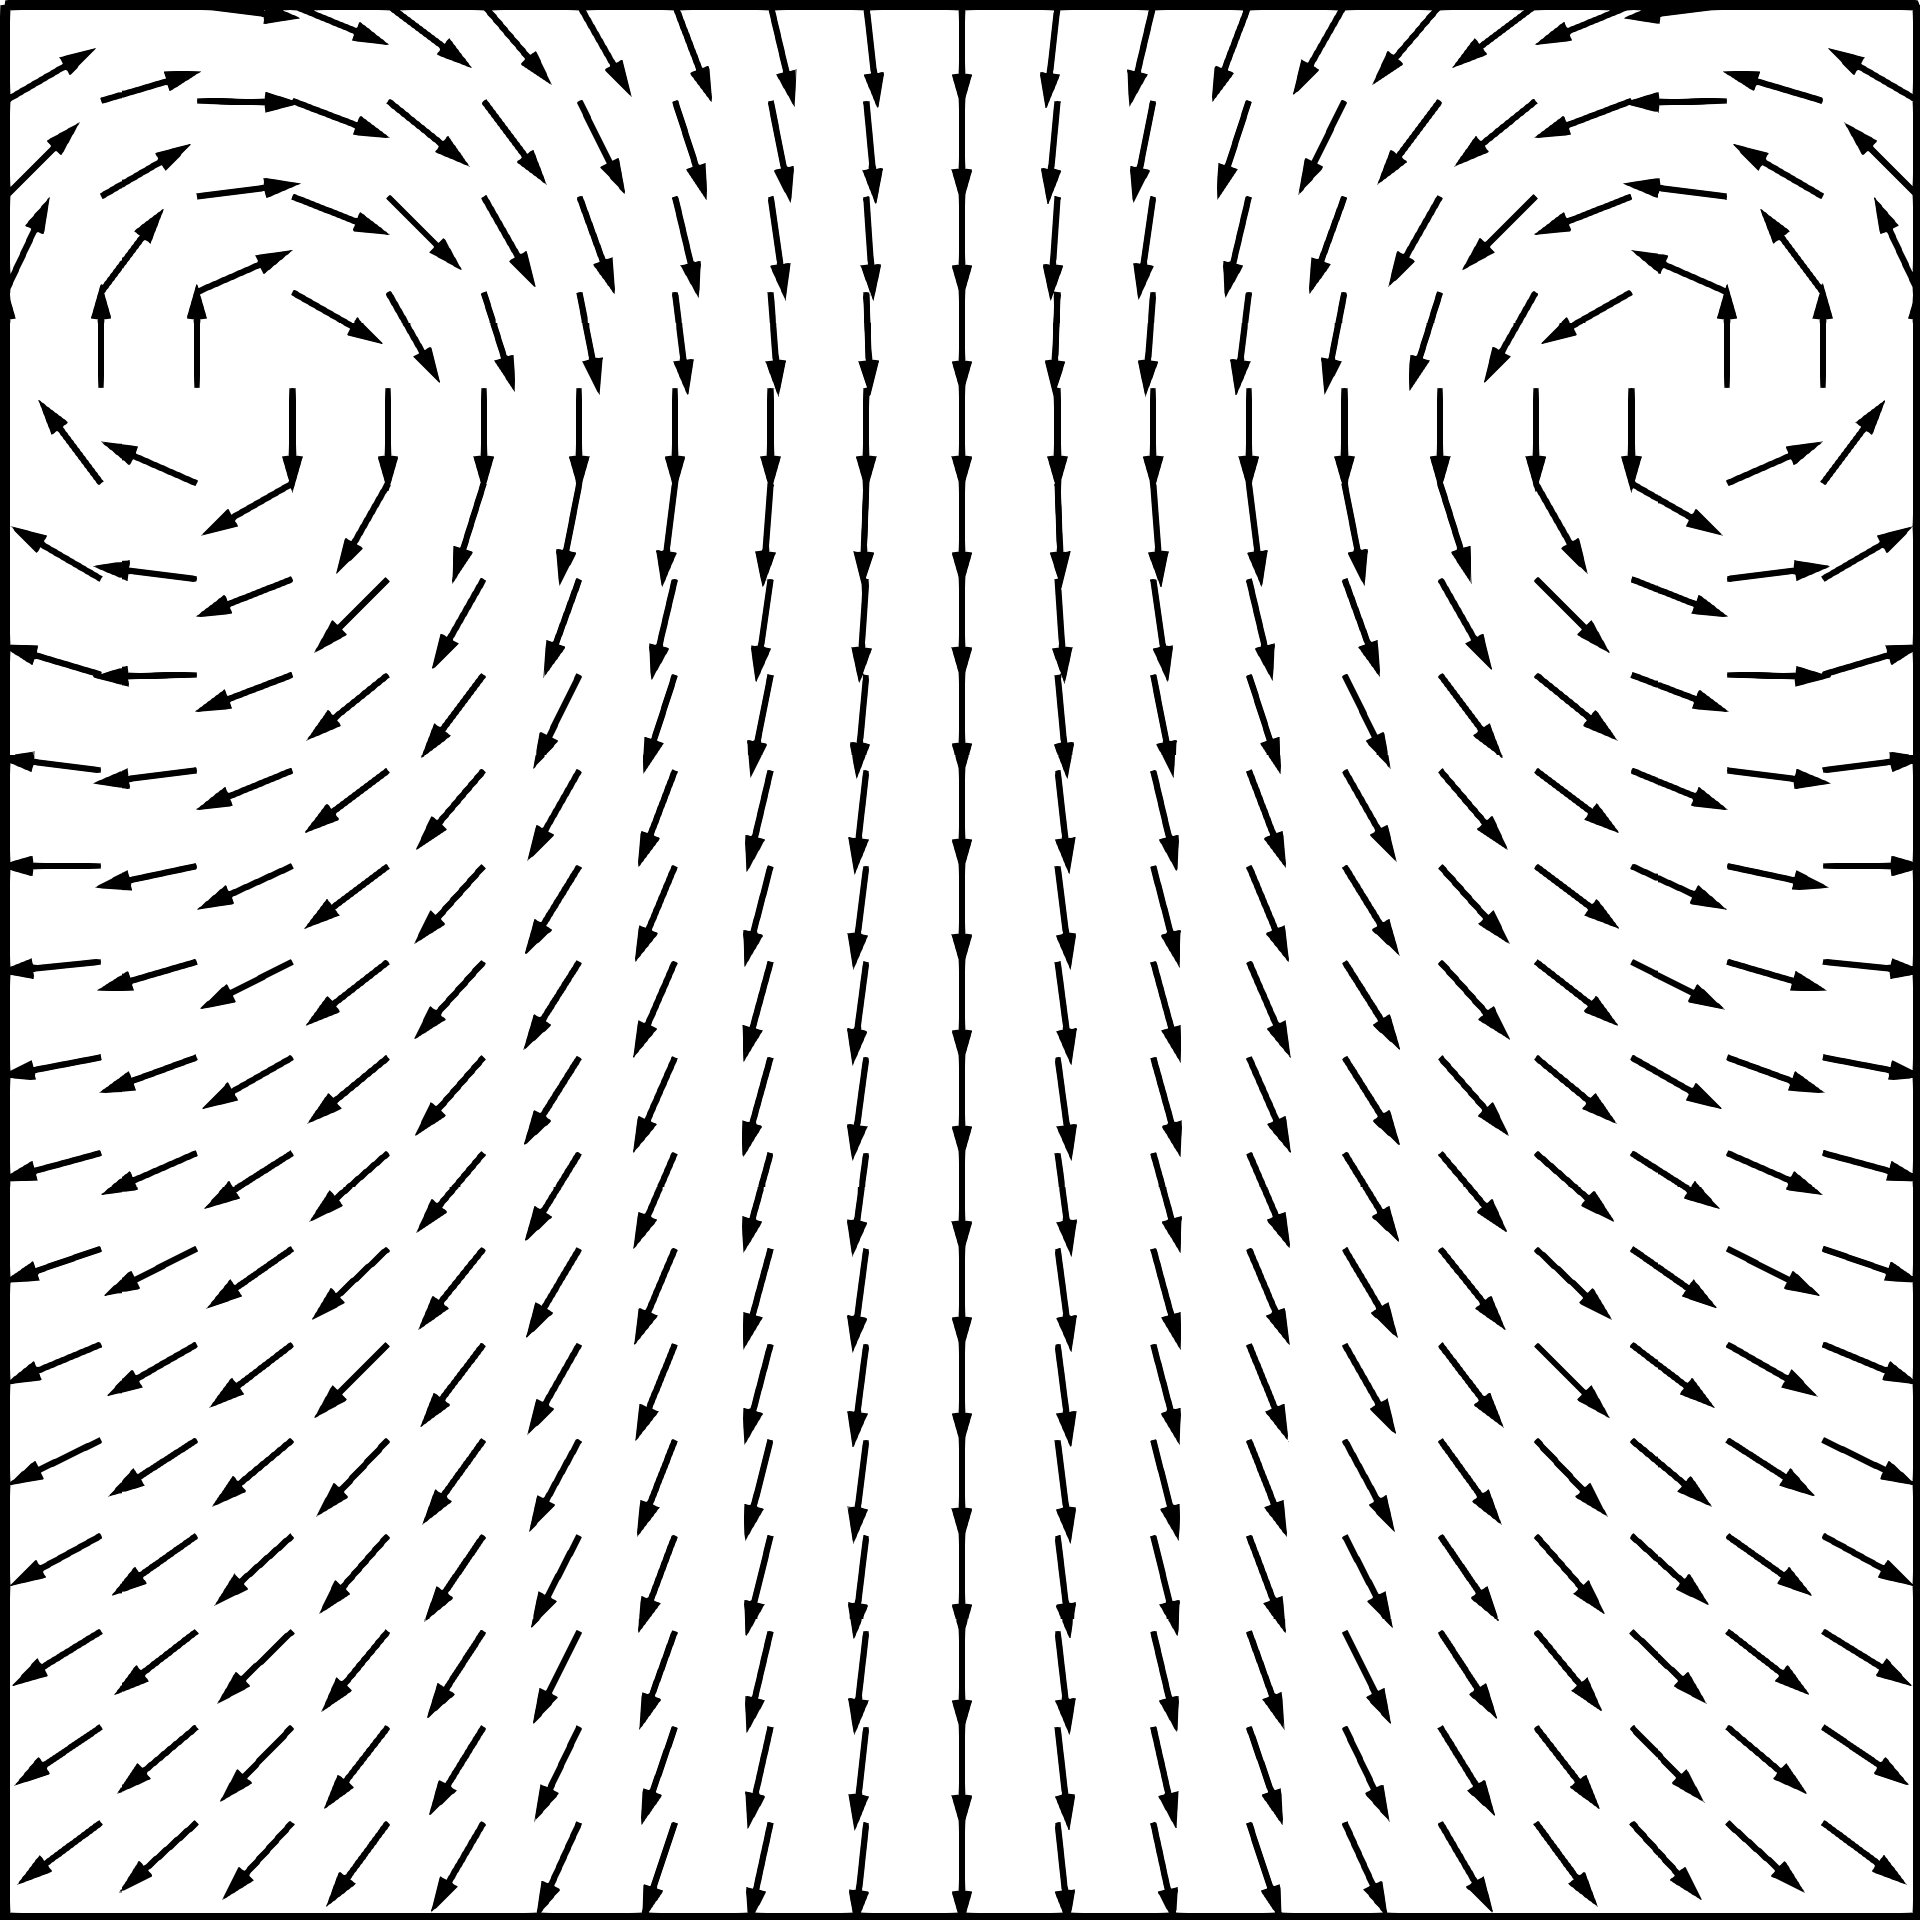
\includegraphics[scale=.065]{figures/Coaxing/Glyphs.png}
        \caption{}
    \end{subfigure}
    \begin{subfigure}{.24\textwidth}
        \centering
        
\includegraphics[scale=.065]{figures/Coaxing/SingleLine0.png}
        \caption{}
    \end{subfigure}
    \begin{subfigure}{.24\textwidth}
        \centering
        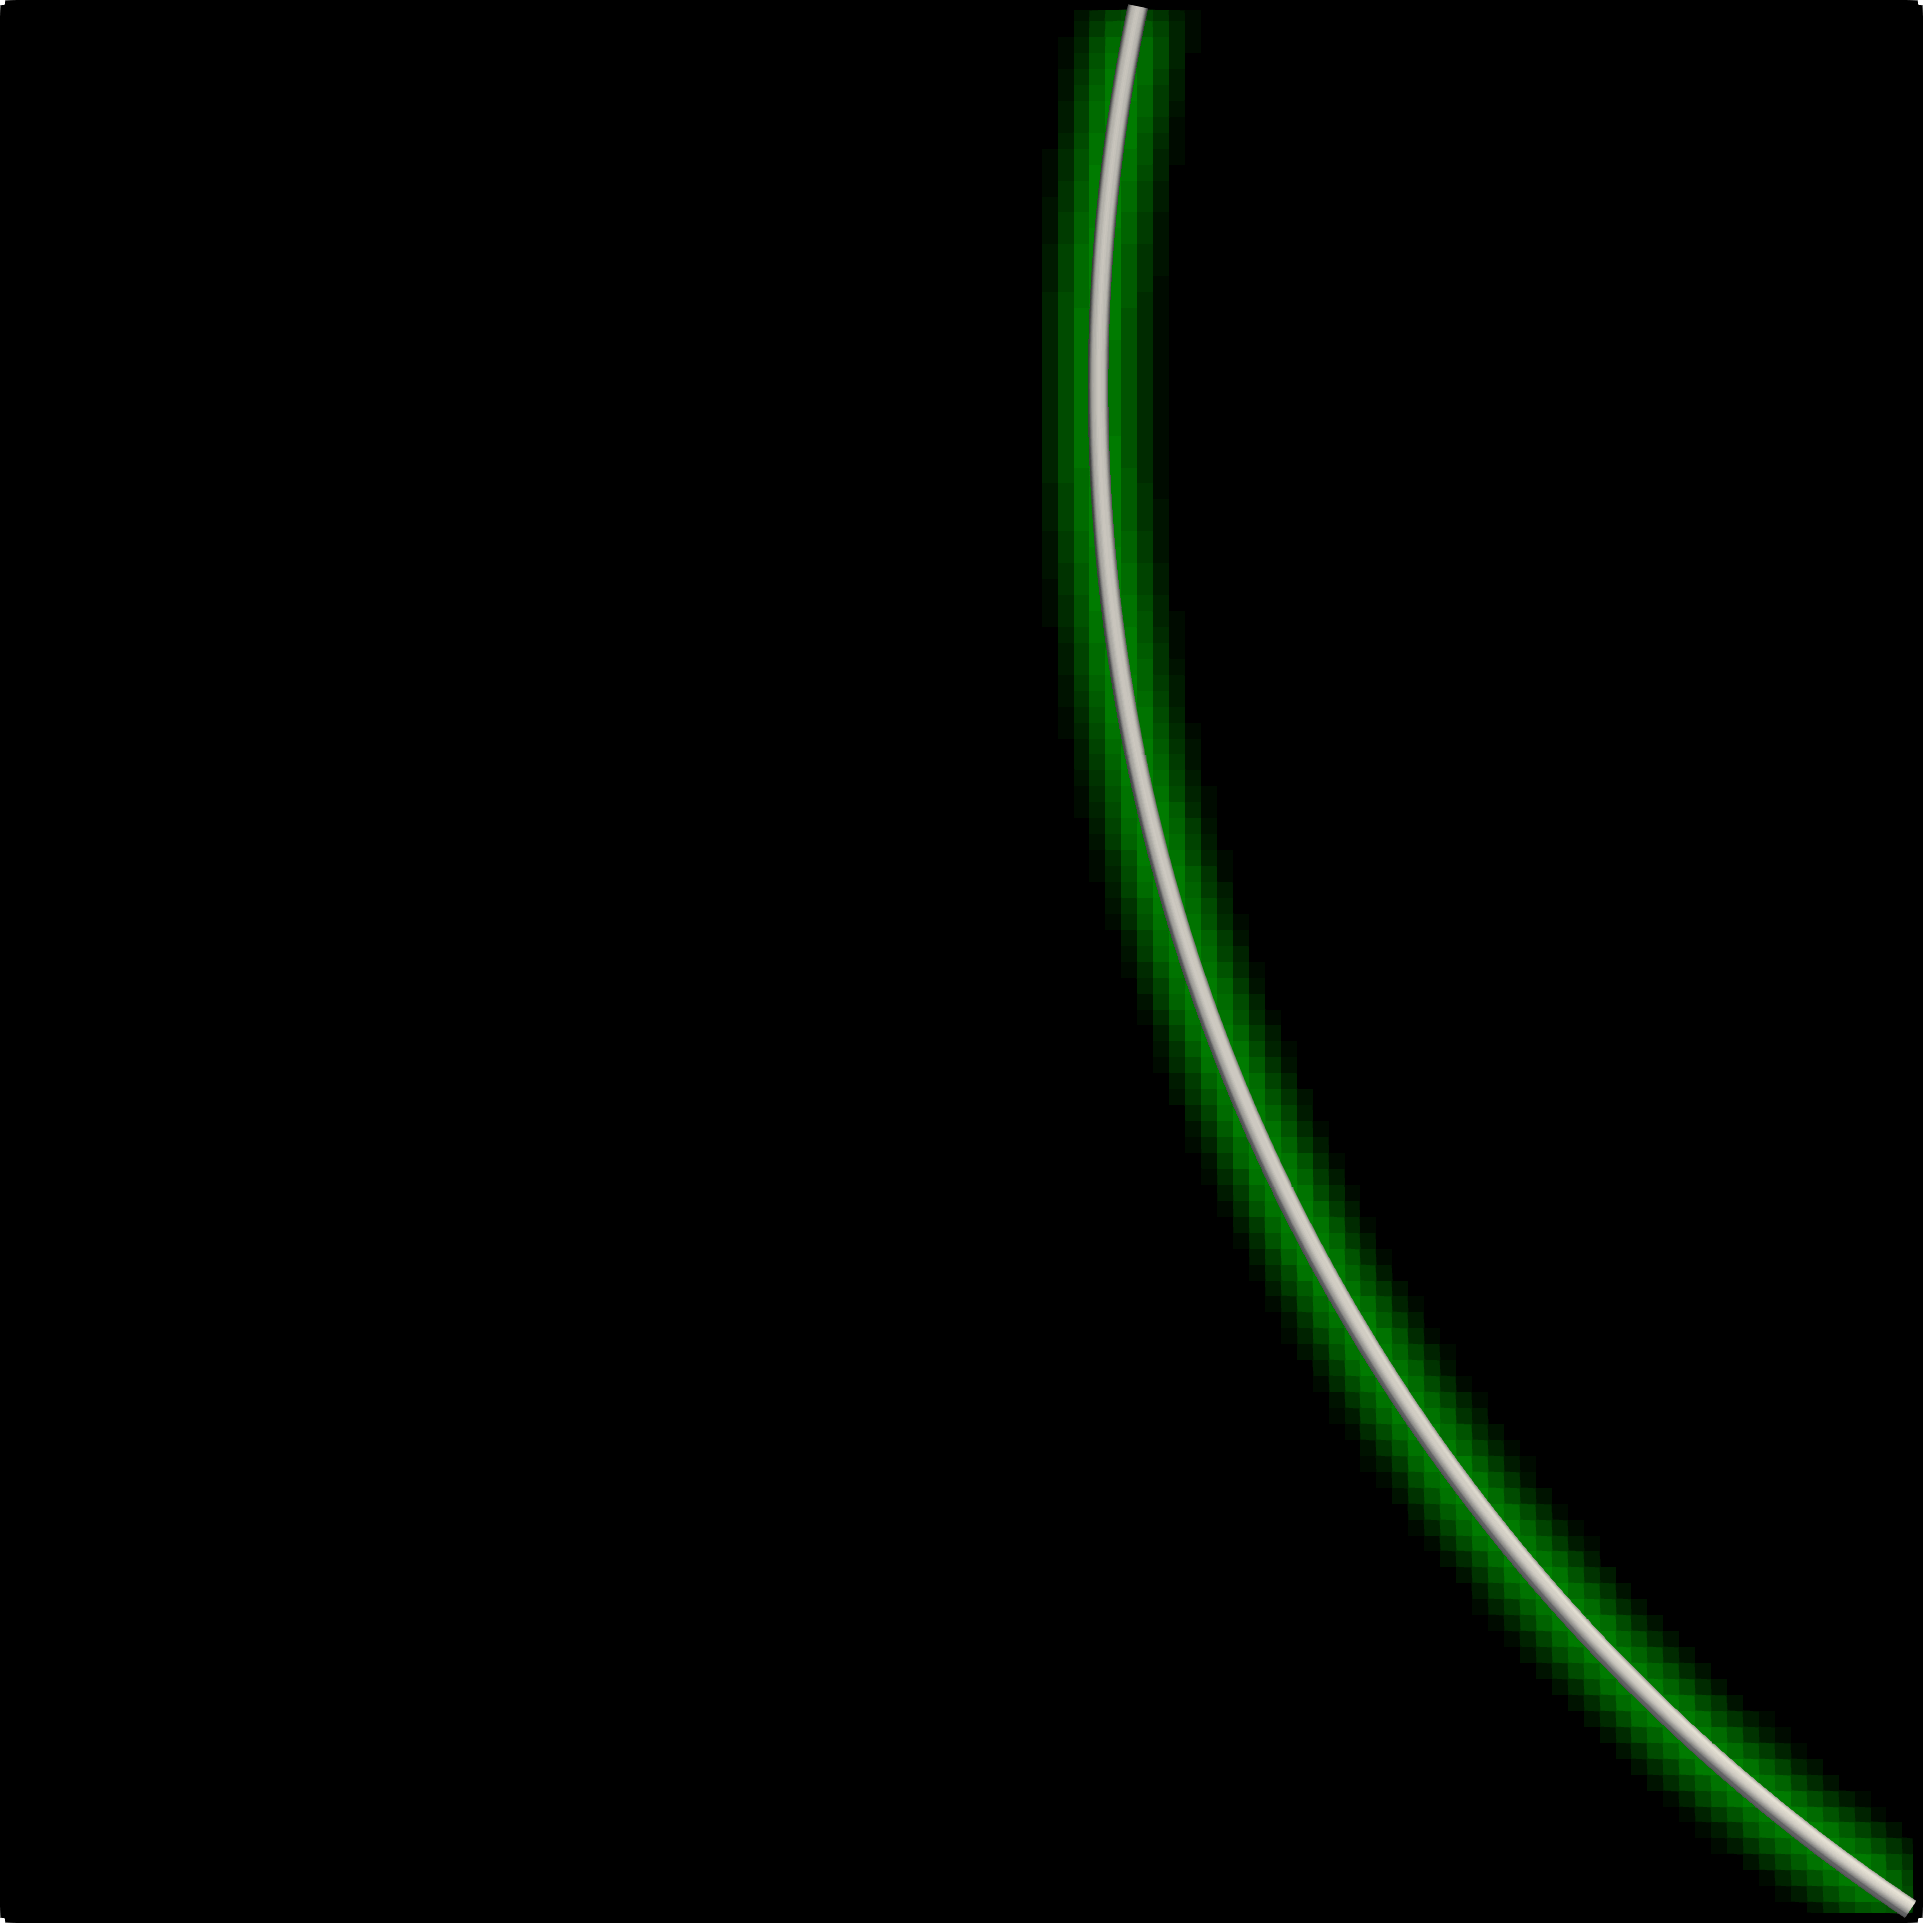
\includegraphics[scale=.065]{figures/Coaxing/SingleLine1.png}
        \caption{}
    \end{subfigure}
    \begin{subfigure}{.24\textwidth}
        \centering
        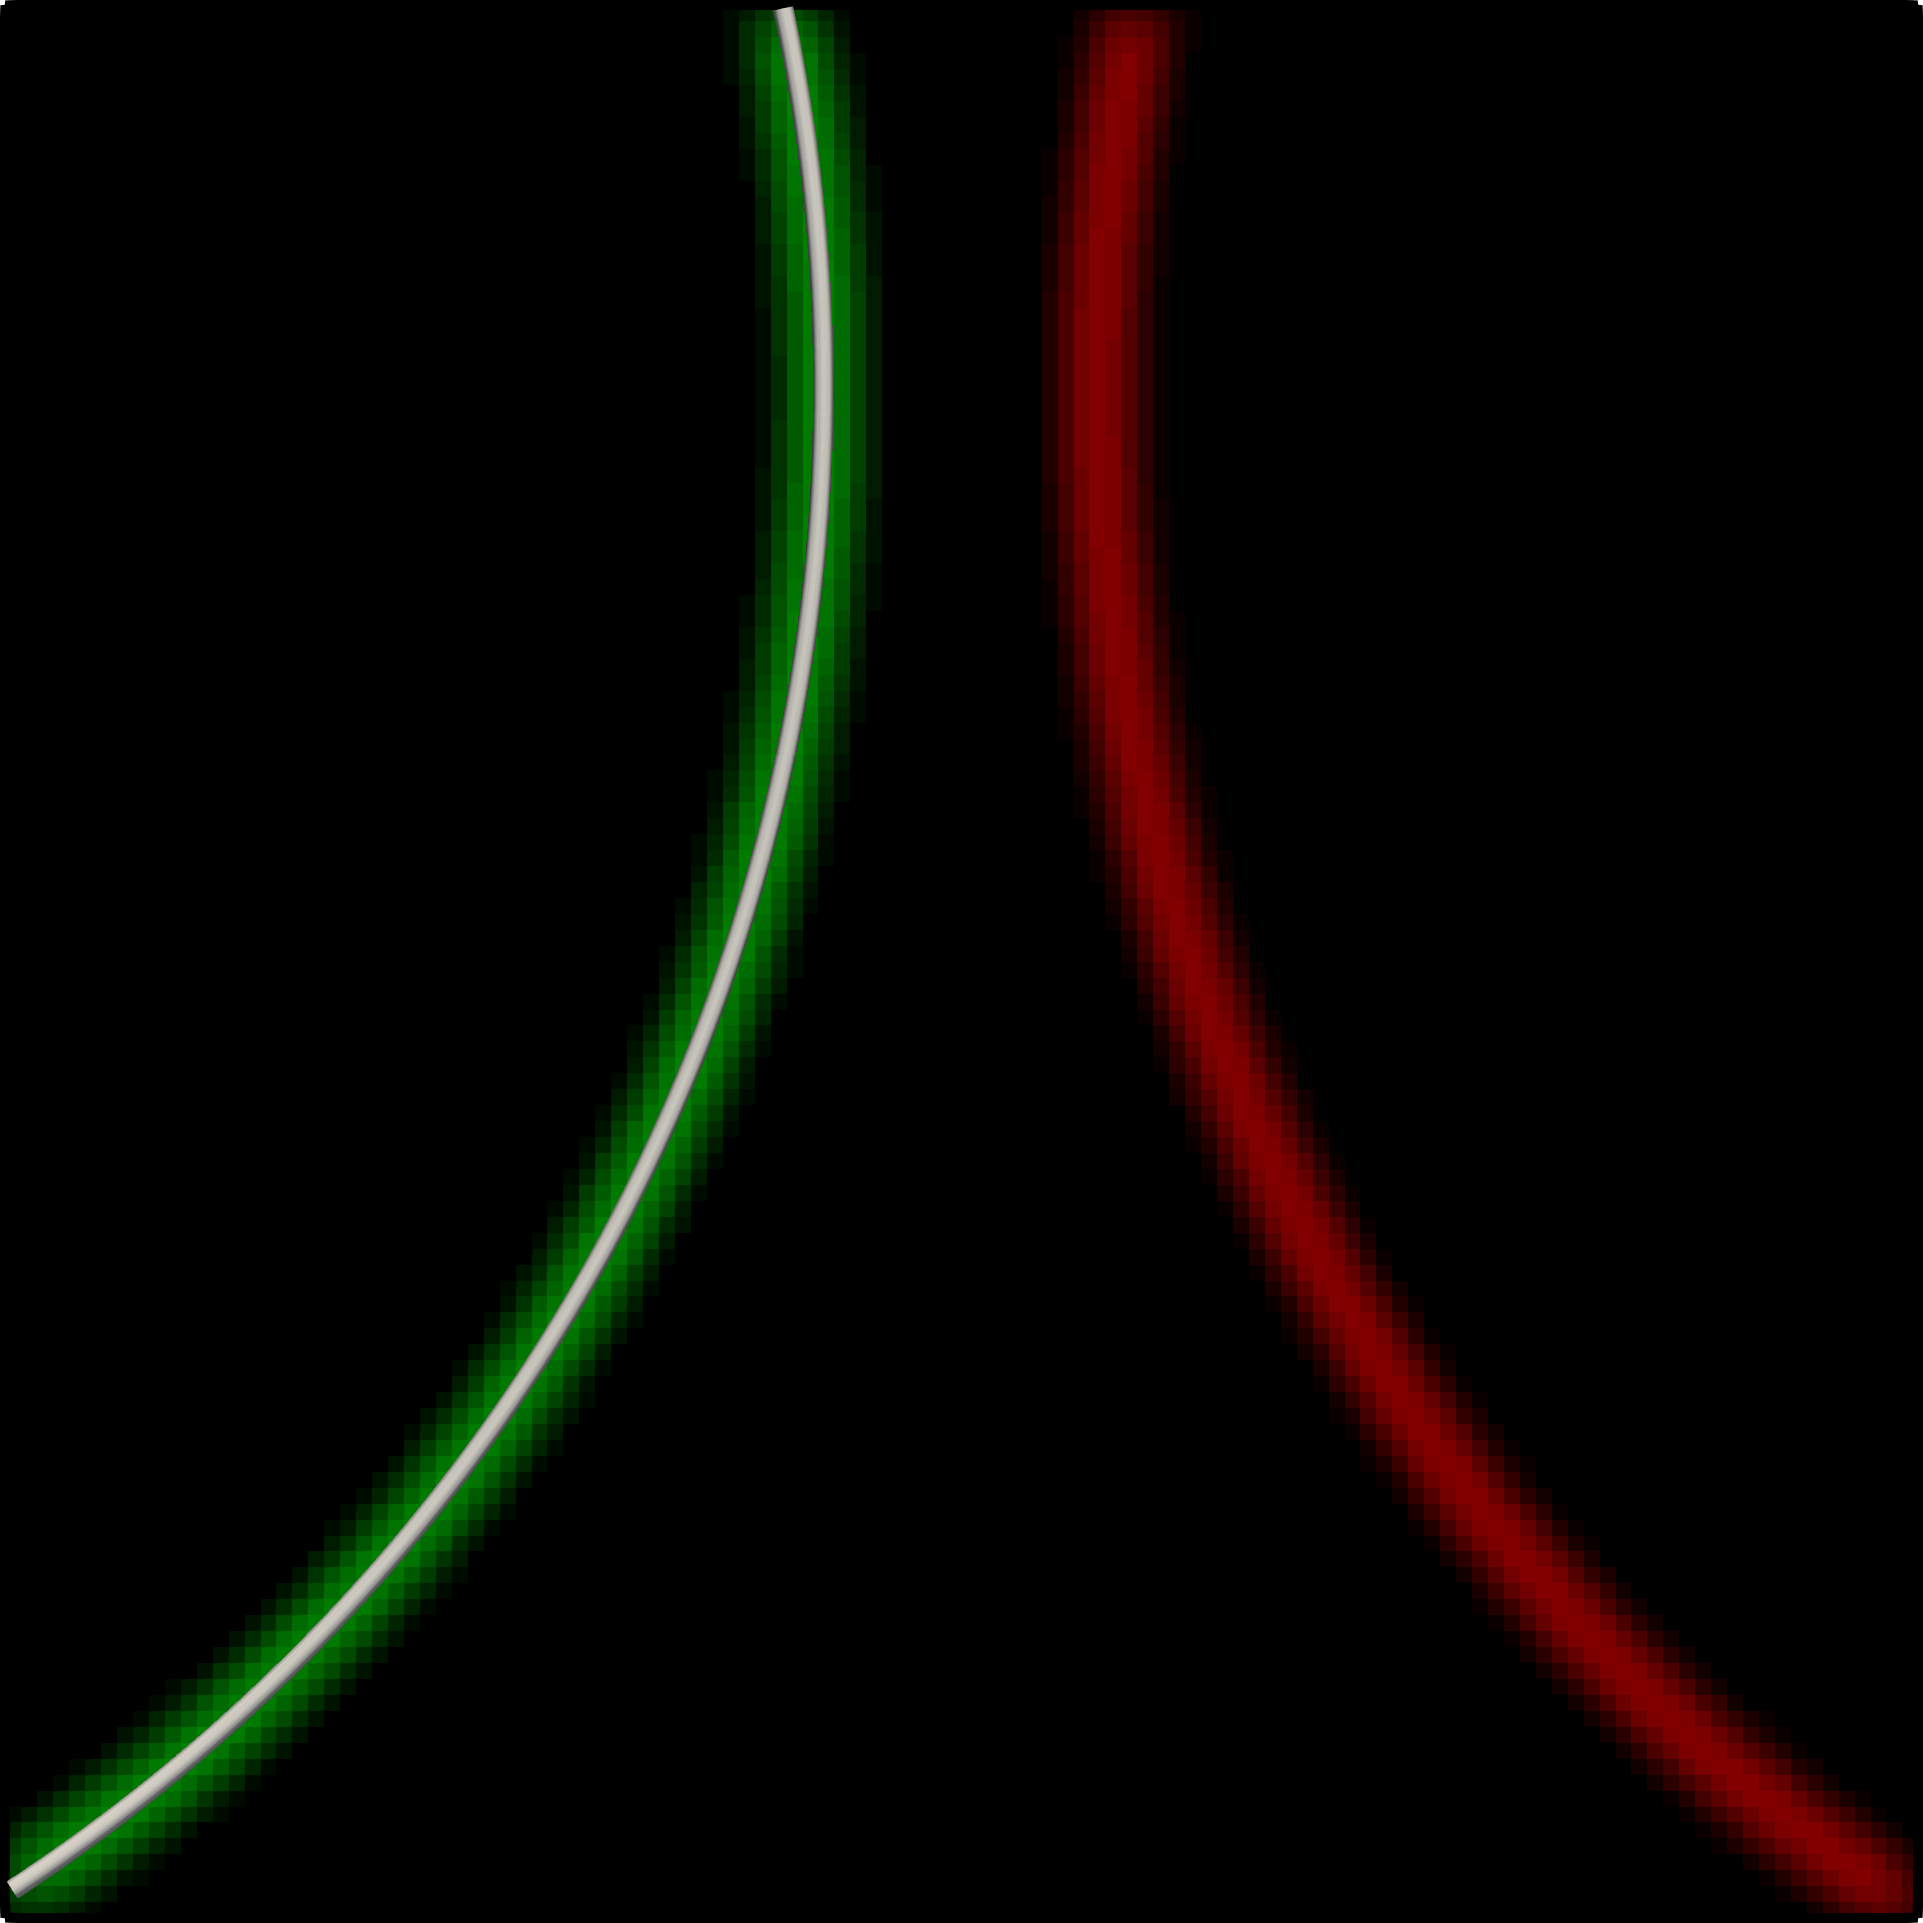
\includegraphics[scale=.065]{figures/Coaxing/SingleLine2.png}
        \caption{}
    \end{subfigure}
    \caption{
        Streamlines may diverge from the same origin when using $\alpha=0$. The field in this figure is $steady$.
        (a) We use the double gyre to show divergent behavior in (d), visualized with an arrow plot.
        (b) Initial seed and starting streamline length.
        (c) Random move and lengthen steps reach a local minimum energy by increasing the streamline length, converging to one side at random.
        (d) A different result may occur with the same starting conditions.
    }
    \label[figure]{fig:energydevelopment}
\end{figure}
Since we compare many images and footprints from this section onward, it is useful to include a distinction using different color channels.
For the rest of this thesis, we use a consistent coloring to show streamline movement between time frames.
Footprints from the current frame's streamlines are drawn in green, those from the last step in red.
The higher the intensity of a pixel, the stronger the energy in that region.
High time coherence therefore leads to most of the image being yellow, with few red or green areas.
We only draw the footprints obtained using the filter $L_t$, as those from $L_s$ can be easily inferred while
$L_t$ provides more visual clarity due to the reduced blur radius.
\begin{leftbar}
    \textbf{Note}: The algorithm may perform a combination of move and lengthen operations at once.
    Even with a constant field, it is possible for streamlines to move or change their length slightly due to this inherent randomness.
    % Nonetheless, this section will give an accurate overview of how changing $\alpha$ impacts image quality.
\end{leftbar}

We now take a closer look at the energy development for different streamline positions
seen in \Cref{fig:energydevelopment} (a--d).
We start with a simple, steady field shown in (a), and a constant starting position for
every execution at the center (b).
After 100 optimization steps, the streamline has grown to the maximum length possible (c),
thereby reaching a minimum in spatial energy.
(d) shows the two likely outcomes of how the starting streamline develops under the specified starting conditions.
Due to the randomness of the algorithm, there is a $\approx50\,\%$ chance of ending up on either side of the center ridge (d).
\newpage

\begin{figure}[ht]
    \begin{subfigure}{\textwidth}
        \begin{subfigure}{.33\textwidth}
            \centering
            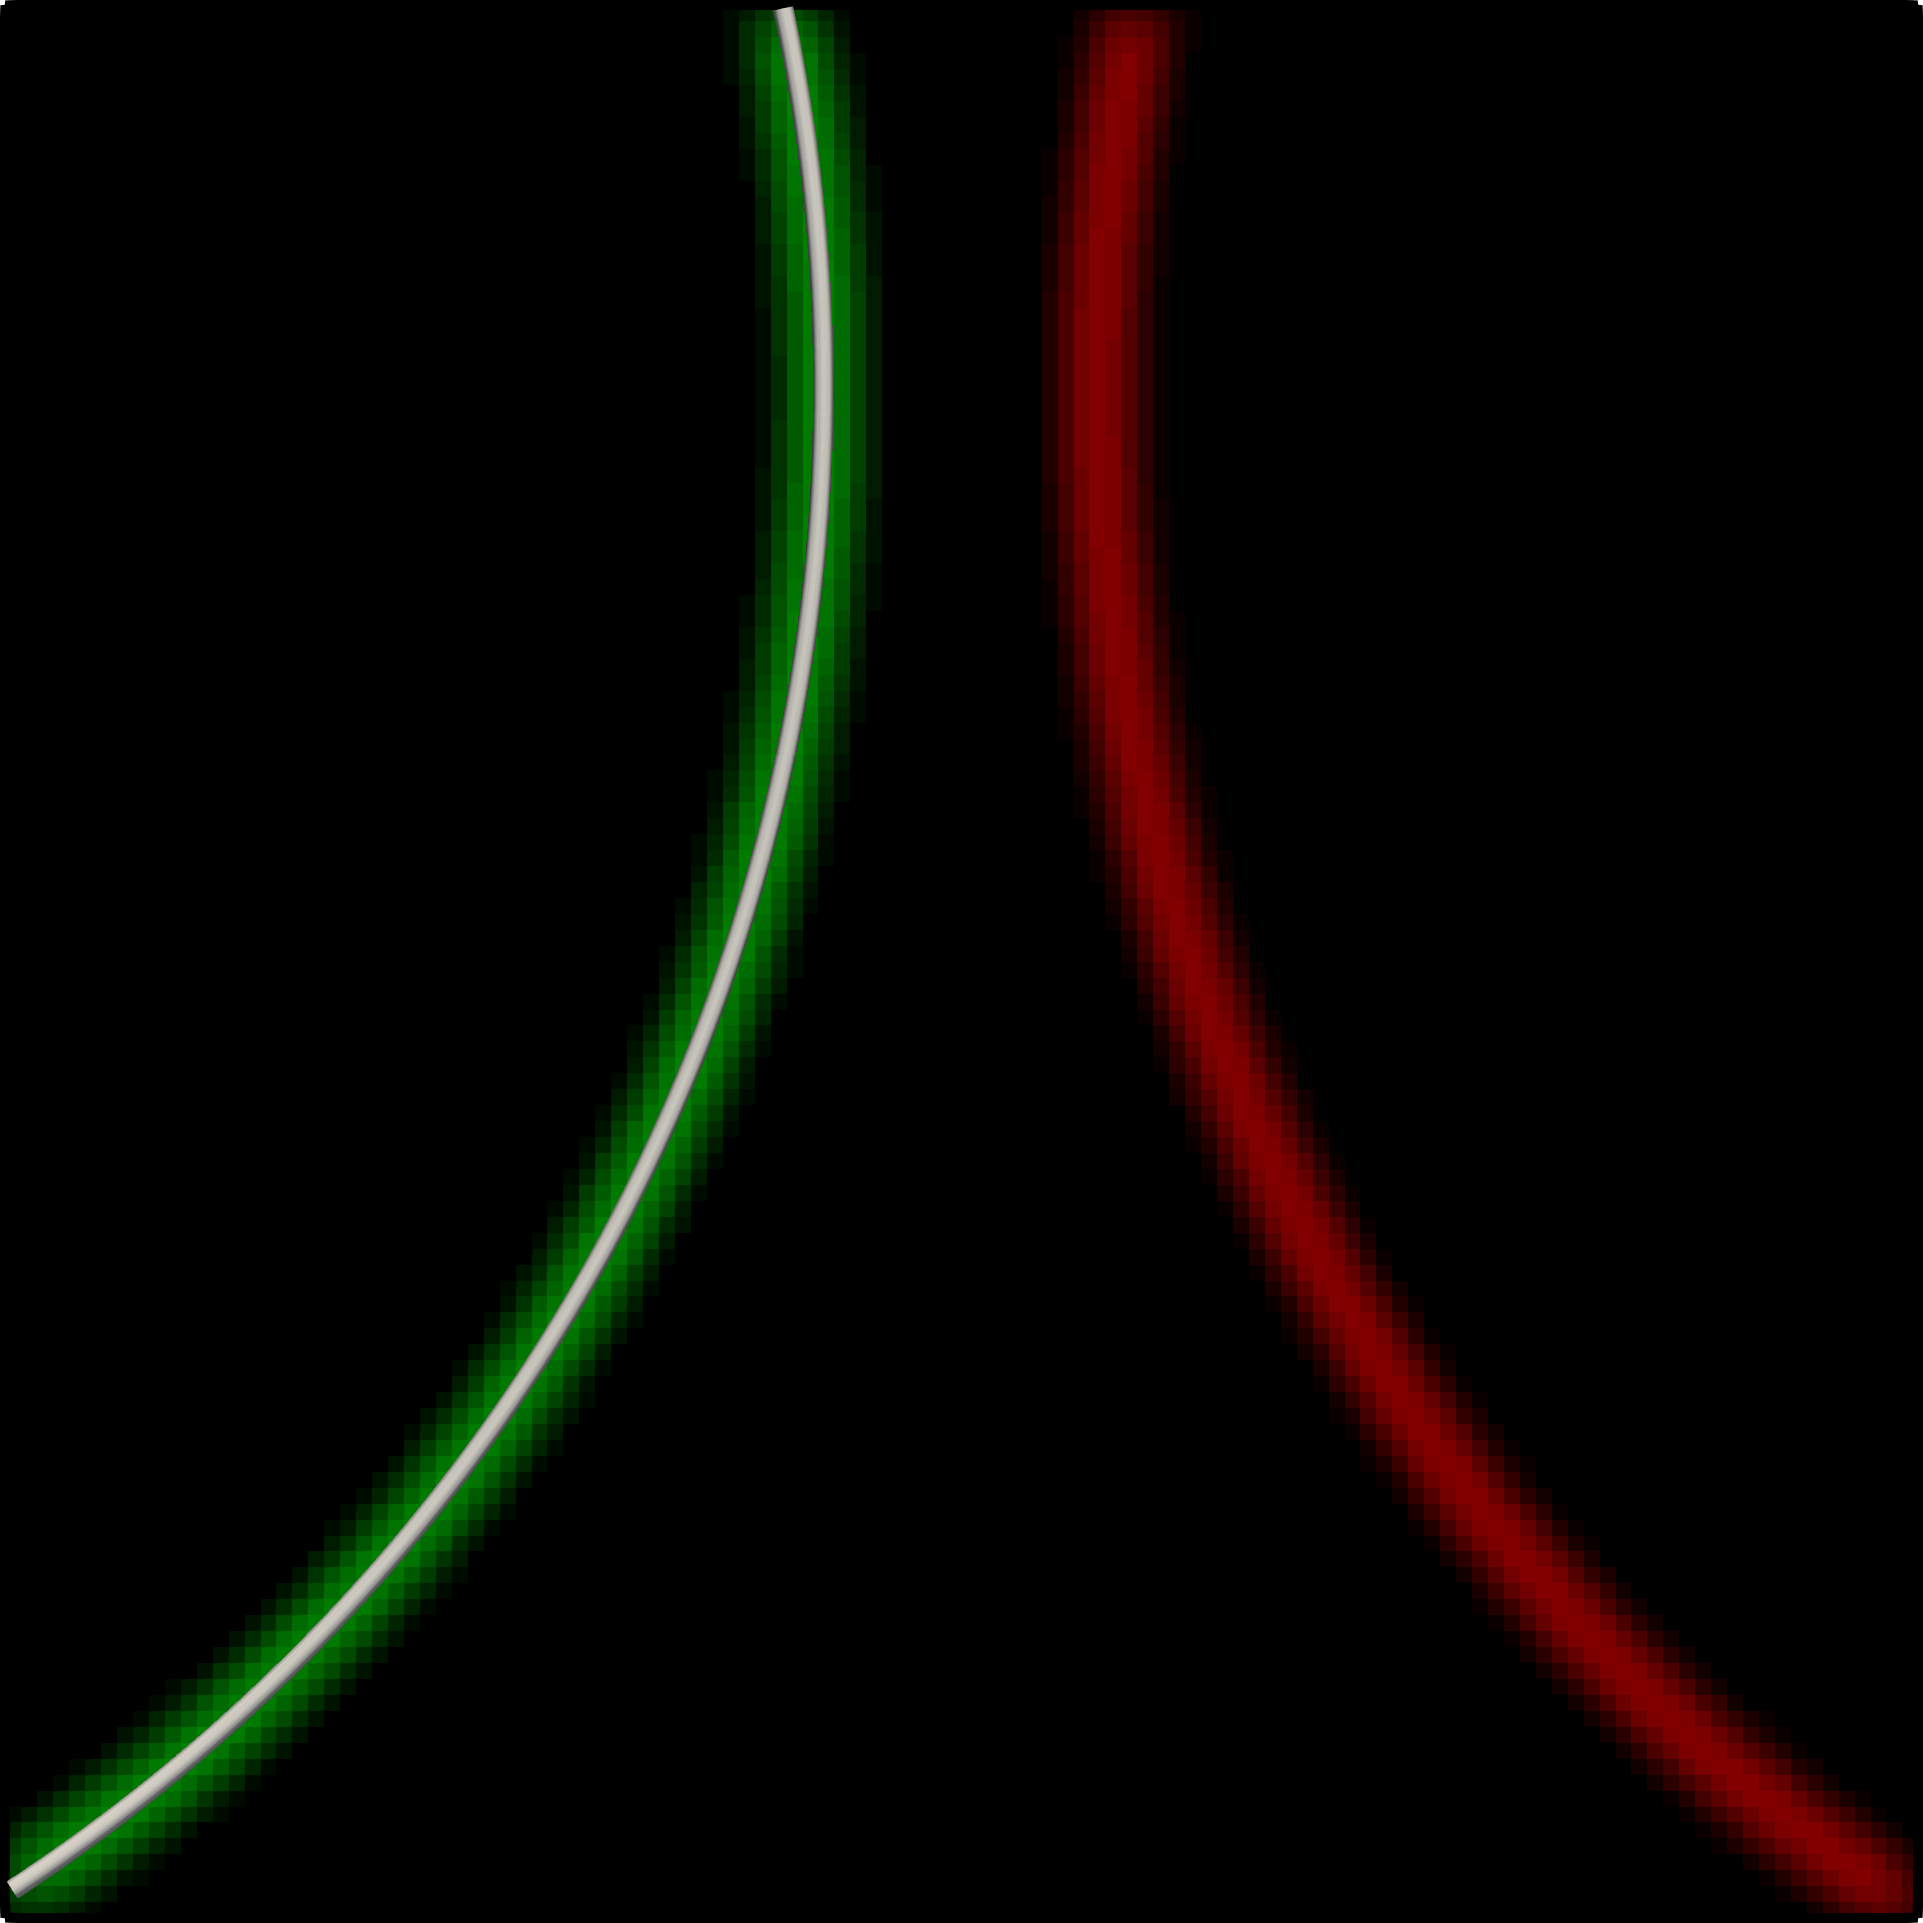
\includegraphics[scale=.06]{figures/Coaxing/SingleLine2.png}
            \caption*{\textbf{(a)}}
        \end{subfigure}
        \begin{subfigure}{.65\textwidth}
            \centering
            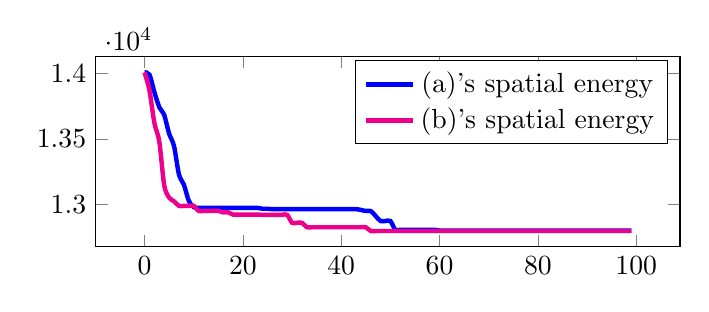
\begin{tikzpicture}
    \begin{axis} [
        width=9cm,
        height=4cm,
        every axis plot post/.append style={ultra thick, mark=none},
        xlabel=,
        ylabel=,
        x tick scale label style={},
    ]
        % Separate        
        \addplot +[smooth] [color=blue] coordinates {
            (0, 14007.826)
            (1, 13989.577)
            (2, 13856.987)
            (3, 13741.918)
            (4, 13681.778)
            (5, 13540.625)
            (6, 13445.154)
            (7, 13229.154)
            (8, 13151.793)
            (9, 13028.149)
            (10, 12979.961)
            (11, 12974.256)
            (12, 12974.256)
            (13, 12974.256)
            (14, 12974.256)
            (15, 12974.256)
            (16, 12974.256)
            (17, 12974.256)
            (18, 12974.256)
            (19, 12974.256)
            (20, 12974.256)
            (21, 12974.256)
            (22, 12974.256)
            (23, 12974.256)
            (24, 12968.2)
            (25, 12968.2)
            (26, 12965.026)
            (27, 12965.026)
            (28, 12965.026)
            (29, 12965.026)
            (30, 12965.026)
            (31, 12965.026)
            (32, 12965.026)
            (33, 12965.026)
            (34, 12965.026)
            (35, 12965.026)
            (36, 12965.026)
            (37, 12965.026)
            (38, 12965.026)
            (39, 12965.026)
            (40, 12965.026)
            (41, 12965.026)
            (42, 12965.026)
            (43, 12965.026)
            (44, 12959.116)
            (45, 12950.877)
            (46, 12950.877)
            (47, 12912.311)
            (48, 12874.413)
            (49, 12874.413)
            (50, 12874.413)
            (51, 12807.514)
            (52, 12807.514)
            (53, 12807.514)
            (54, 12807.514)
            (55, 12807.514)
            (56, 12807.514)
            (57, 12807.514)
            (58, 12807.514)
            (59, 12807.514)
            (60, 12801.792)
            (61, 12801.792)
            (62, 12801.792)
            (63, 12801.792)
            (64, 12801.289)
            (65, 12801.289)
            (66, 12801.289)
            (67, 12801.289)
            (68, 12801.289)
            (69, 12801.289)
            (70, 12801.289)
            (71, 12801.289)
            (72, 12801.289)
            (73, 12801.289)
            (74, 12801.289)
            (75, 12801.289)
            (76, 12801.289)
            (77, 12801.289)
            (78, 12801.289)
            (79, 12801.289)
            (80, 12801.289)
            (81, 12801.289)
            (82, 12801.289)
            (83, 12801.289)
            (84, 12801.289)
            (85, 12801.289)
            (86, 12801.289)
            (87, 12801.289)
            (88, 12801.289)
            (89, 12801.289)
            (90, 12801.289)
            (91, 12801.289)
            (92, 12801.289)
            (93, 12801.289)
            (94, 12801.289)
            (95, 12801.289)
            (96, 12801.289)
            (97, 12801.289)
            (98, 12801.289)
            (99, 12801.289)
        };
        % Overlapping
        \addplot +[smooth] [color=magenta] coordinates {
            (0, 14007.826) 
            (1, 13869.016) 
            (2, 13622.305) 
            (3, 13479.086) 
            (4, 13146.85)  
            (5, 13052.909) 
            (6, 13024.708) 
            (7, 12989.768) 
            (8, 12989.768) 
            (9, 12989.768) 
            (10, 12989.768)
            (11, 12951.466)
            (12, 12951.466)
            (13, 12951.466)
            (14, 12951.466)
            (15, 12951.466)
            (16, 12940.784)
            (17, 12940.784)
            (18, 12923.523)
            (19, 12923.523)
            (20, 12923.523)
            (21, 12923.523)
            (22, 12923.523)
            (23, 12923.523)
            (24, 12921.698)
            (25, 12921.698)
            (26, 12921.698)
            (27, 12921.698)
            (28, 12921.698)
            (29, 12921.698)
            (30, 12860.99) 
            (31, 12860.99) 
            (32, 12860.99)
            (33, 12827.076)
            (34, 12827.076)
            (35, 12827.076)
            (36, 12827.076)
            (37, 12827.076)
            (38, 12827.076)
            (39, 12827.076)
            (40, 12827.076)
            (41, 12827.076)
            (42, 12827.076)
            (43, 12827.076)
            (44, 12827.076)
            (45, 12827.076)
            (46, 12798.14)
            (47, 12798.14)
            (48, 12798.14)
            (49, 12798.14)
            (50, 12798.14)
            (51, 12798.14)
            (52, 12798.14)
            (53, 12798.14)
            (54, 12798.14)
            (55, 12798.14)
            (56, 12798.14)
            (57, 12798.14)
            (58, 12798.14)
            (59, 12798.14)
            (60, 12798.14)
            (61, 12798.14)
            (62, 12798.14)
            (63, 12798.14)
            (64, 12798.14)
            (65, 12798.14)
            (66, 12798.14)
            (67, 12798.14)
            (68, 12798.14)
            (69, 12798.14)
            (70, 12798.14)
            (71, 12798.14)
            (72, 12798.14)
            (73, 12798.14)
            (74, 12798.14)
            (75, 12798.14)
            (76, 12798.14)
            (77, 12798.14)
            (78, 12798.14)
            (79, 12798.14)
            (80, 12798.14)
            (81, 12798.14)
            (82, 12798.14)
            (83, 12798.14)
            (84, 12798.14)
            (85, 12798.14)
            (86, 12798.14)
            (87, 12798.14)
            (88, 12798.14)
            (89, 12798.14)
            (90, 12798.14)
            (91, 12798.14)
            (92, 12798.14)
            (93, 12798.14)
            (94, 12798.14)
            (95, 12798.14)
            (96, 12798.14)
            (97, 12798.14)
            (98, 12798.14)
            (99, 12798.14)
        };
        \addlegendentry{(a)'s spatial energy}
        \addlegendentry{(b)'s spatial energy}
    \end{axis}
\end{tikzpicture}

            \caption*{\textbf{(c)}}
        \end{subfigure}
    \end{subfigure}
    \begin{subfigure}{\textwidth}
        \begin{subfigure}{.33\textwidth}
            \centering
            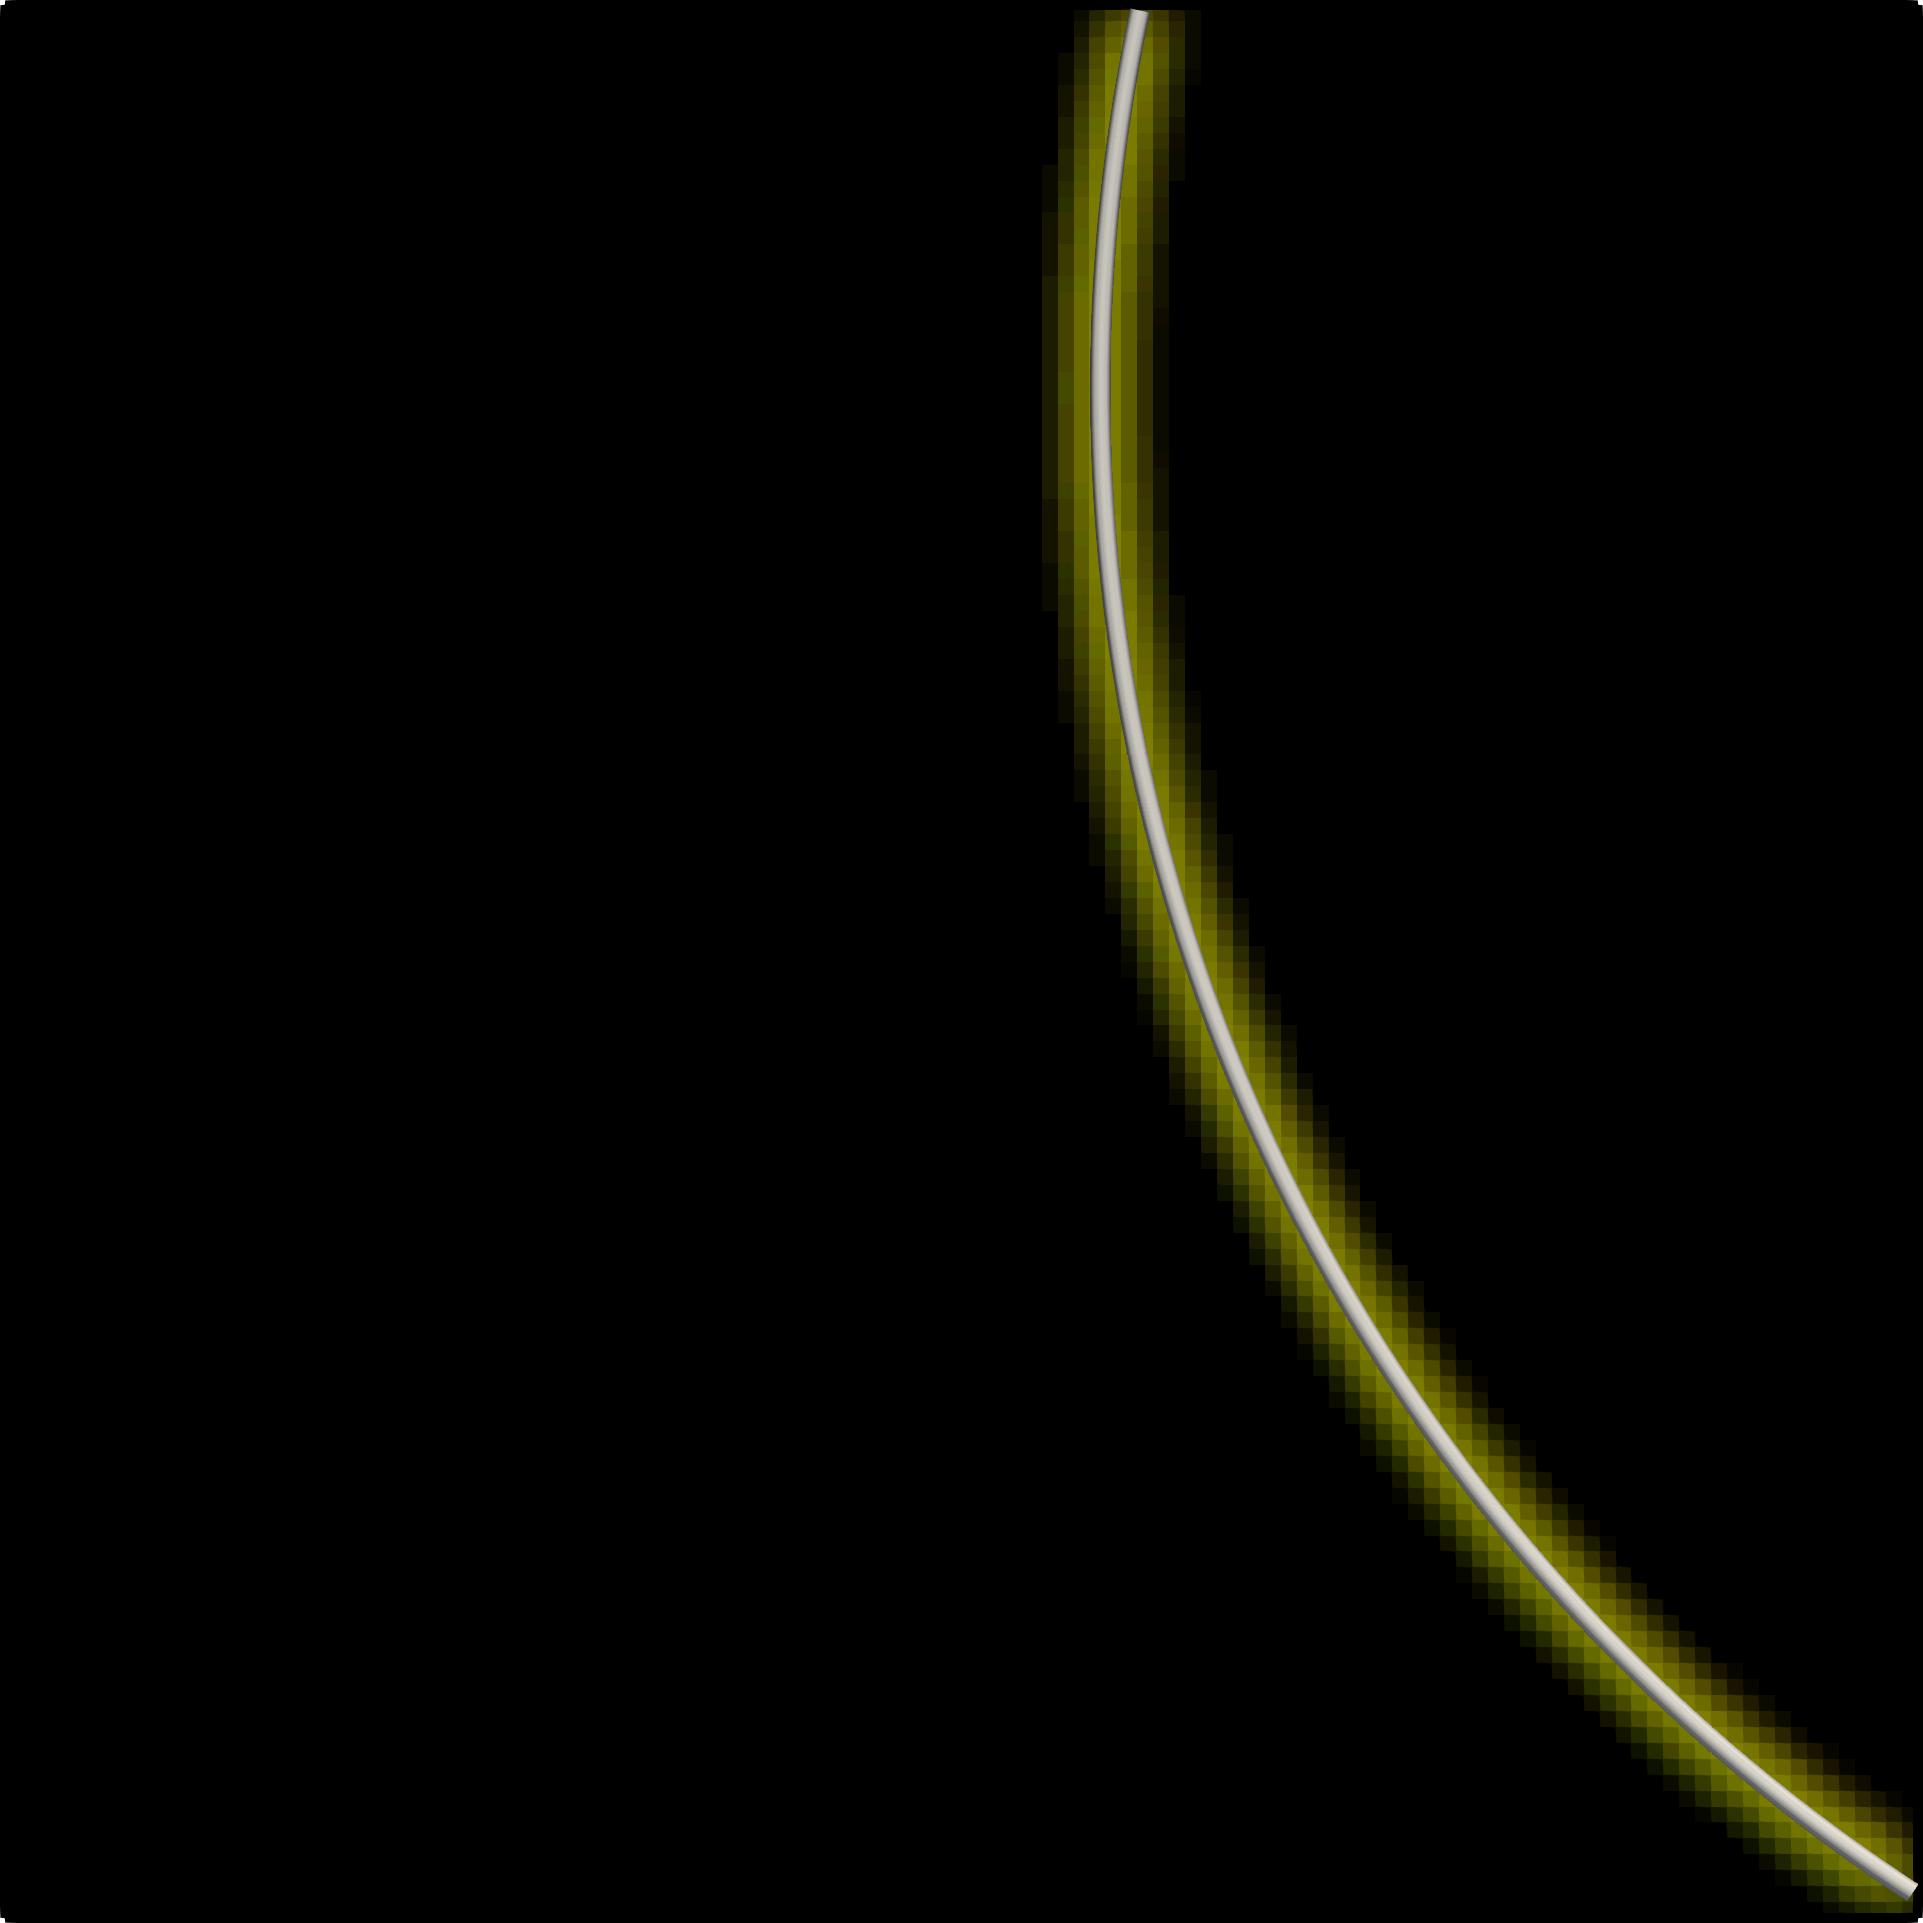
\includegraphics[scale=.06]{figures/Coaxing/SingleLineC1.png}
            \caption*{\textbf{(b)}}
        \end{subfigure}
        \begin{subfigure}{.65\textwidth}
            \centering
            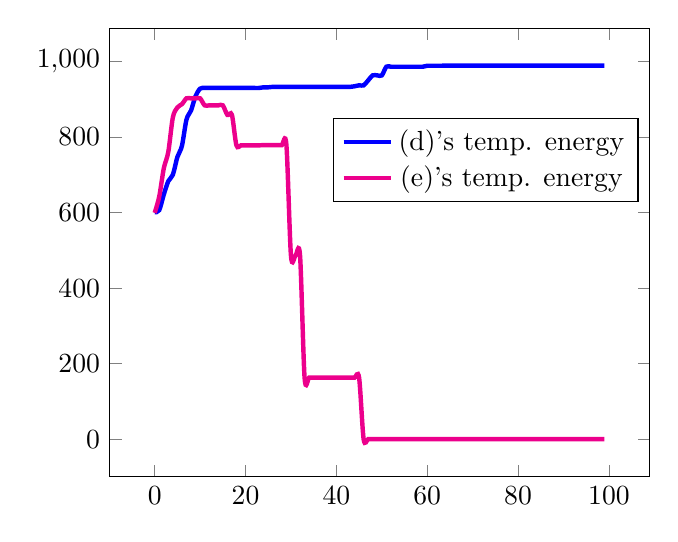
\begin{tikzpicture}
    \begin{axis} [
        every axis plot post/.append style={ultra thick, mark=none}, 
        xlabel=,
        legend style={at={(.98,.8)},anchor=north east}
    ]
        \addplot +[smooth] [color=blue] coordinates {
            (0, 600.738)
            (1, 606.401)
            (2, 647.542)
            (3, 683.247)
            (4, 700.14)
            (5, 747.113)
            (6, 776.618)
            (7, 846.143)
            (8, 870.048)
            (9, 908.393)
            (10, 928.066)
            (11, 929.862)
            (12, 929.862)
            (13, 929.862)
            (14, 929.862)
            (15, 929.862)
            (16, 929.862)
            (17, 929.862)
            (18, 929.862)
            (19, 929.862)
            (20, 929.862)
            (21, 929.862)
            (22, 929.862)
            (23, 929.862)
            (24, 931.591)
            (25, 931.591)
            (26, 932.786)
            (27, 932.786)
            (28, 932.786)
            (29, 932.786)
            (30, 932.786)
            (31, 932.786)
            (32, 932.786)
            (33, 932.786)
            (34, 932.786)
            (35, 932.786)
            (36, 932.786)
            (37, 932.786)
            (38, 932.786)
            (39, 932.786)
            (40, 932.786)
            (41, 932.786)
            (42, 932.786)
            (43, 932.786)
            (44, 934.333)
            (45, 936.797)
            (46, 936.797)
            (47, 949.954)
            (48, 963.133)
            (49, 963.133)
            (50, 963.133)
            (51, 986.039)
            (52, 986.039)
            (53, 986.039)
            (54, 986.039)
            (55, 986.039)
            (56, 986.039)
            (57, 986.039)
            (58, 986.039)
            (59, 986.039)
            (60, 988.596)
            (61, 988.596)
            (62, 988.596)
            (63, 988.596)
            (64, 989.078)
            (65, 989.078)
            (66, 989.078)
            (67, 989.078)
            (68, 989.078)
            (69, 989.078)
            (70, 989.078)
            (71, 989.078)
            (72, 989.078)
            (73, 989.078)
            (74, 989.078)
            (75, 989.078)
            (76, 989.078)
            (77, 989.078)
            (78, 989.078)
            (79, 989.078)
            (80, 989.078)
            (81, 989.078)
            (82, 989.078)
            (83, 989.078)
            (84, 989.078)
            (85, 989.078)
            (86, 989.078)
            (87, 989.078)
            (88, 989.078)
            (89, 989.078)
            (90, 989.078)
            (91, 989.078)
            (92, 989.078)
            (93, 989.078)
            (94, 989.078)
            (95, 989.078)
            (96, 989.078)
            (97, 989.078)
            (98, 989.078)
            (99, 989.078)    
        };
        \addplot +[smooth] [color=magenta] coordinates {
            (0, 599.266) 
            (1, 642.339) 
            (2, 716.691) 
            (3, 760.73)  
            (4, 851.884) 
            (5, 878.242) 
            (6, 886.961) 
            (7, 902.354) 
            (8, 902.354) 
            (9, 902.354) 
            (10, 902.354)
            (11, 883.831)
            (12, 883.831)
            (13, 883.831)
            (14, 883.831)
            (15, 883.831)
            (16, 858.702)
            (17, 858.702)
            (18, 777.924)
            (19, 777.924)
            (20, 777.924)
            (21, 777.924)
            (22, 777.924)
            (23, 777.924)
            (24, 778.653)
            (25, 778.653)
            (26, 778.653)
            (27, 778.653)
            (28, 778.653)
            (29, 778.653)
            (30, 486.235)
            (31, 486.235)
            (32, 486.235)
            (33, 163.149)
            (34, 163.149)
            (35, 163.149)
            (36, 163.149)
            (37, 163.149)
            (38, 163.149)
            (39, 163.149)
            (40, 163.149)
            (41, 163.149)
            (42, 163.149)
            (43, 163.149)
            (44, 163.149)
            (45, 163.149)
            (46, 0.216)
            (47, 0.216)
            (48, 0.216)
            (49, 0.216)
            (50, 0.216)
            (51, 0.216)
            (52, 0.216)
            (53, 0.216)
            (54, 0.216)
            (55, 0.216)
            (56, 0.216)
            (57, 0.216)
            (58, 0.216)
            (59, 0.216)
            (60, 0.216)
            (61, 0.216)
            (62, 0.216)
            (63, 0.216)
            (64, 0.216)
            (65, 0.216)
            (66, 0.216)
            (67, 0.216)
            (68, 0.216)
            (69, 0.216)
            (70, 0.216)
            (71, 0.216)
            (72, 0.216)
            (73, 0.216)
            (74, 0.216)
            (75, 0.216)
            (76, 0.216)
            (77, 0.216)
            (78, 0.216)
            (79, 0.216)
            (80, 0.216)
            (81, 0.216)
            (82, 0.216)
            (83, 0.216)
            (84, 0.216)
            (85, 0.216)
            (86, 0.216)
            (87, 0.216)
            (88, 0.216)
            (89, 0.216)
            (90, 0.216)
            (91, 0.216)
            (92, 0.216)
            (93, 0.216)
            (94, 0.216)
            (95, 0.216)
            (96, 0.216)
            (97, 0.216)
            (98, 0.216)
            (99, 0.216)   
        };
        \addlegendentry{(d)'s temp. energy}
        \addlegendentry{(e)'s temp. energy}
    \end{axis}
\end{tikzpicture}

            \caption*{\textbf{(d)}}
        \end{subfigure}
    \end{subfigure}
    \caption{
        (a) Two divergent streamlines resulting from the same initial streamlet.
        (b) The line overlap in favor of temporal energy.
        (c) Spatial energy of (a) and (b) vs optimization steps.
        (d) Temporal energy of (a) and (b) vs optimization steps.
    }
\label[figure]{fig:energydevelopment2}
\end{figure}
In \Cref{fig:energydevelopment2} (c), we see a plot of the spatial energy vs the current optimization step.
The maximum spatial energy equals the image resolution at 120x120=14400.
Initially, we see a decline in spatial energy for both curves, caused by the comparatively fast lengthening process.
On average, the streamlines grow about 3\,\% image size per step on both sides.
A plateau phase is reached after $\approx$ 10 steps,
as the streamlines approach the domain boundaries and cannot lengthen further.
Due to random movements, the streamline ends drift along the upper and lower domain borders,
slowly lengthening due to the field's curvature increasing the further outward they move.
A final stronger decline happens at 30 and 50 steps for (a) and (b) respectively, as the curvature is strong enough to allow larger regions to be filled by lengthening again.
The delay between (a) and (b) is caused by the random nature of the algorithm, and is equal if both runs use the same randomization setup.
Our streamlines reach the minimum possible energy of about 12800, with a reduction of $\approx 1600$.
Since the streamline length lies at roughly 140\,px and the filter is about 14\,px wide (note: $L_t$ as shown is half the size of $L_s$),
these spatial energy measures aren't surprising. The temporal energy is shown on plot (d), where we can see a stark difference in the development of (a) and (b).
Many features regarding local rate of change are recognizable in both plots,
e.g. the plateau of (b) centered around the 40 step mark.
The final temporal difference lies at 1000 due to the reduced filter radius.
\newpage

\begin{figure}[ht]
    \centering
    % 5 x No coherence
    \begin{subfigure}{\textwidth}
        \centering
        \begin{subfigure}{.19\textwidth}
            \centering
            \includegraphics[scale=.05]{figures/AlphaStudy/GyroL05.png}
        \end{subfigure}
        \begin{subfigure}{.19\textwidth}
            \centering
            \includegraphics[scale=.05]{figures/AlphaStudy/GyroA03L05.png}
        \end{subfigure}
        \begin{subfigure}{.19\textwidth}
            \centering
            \includegraphics[scale=.05]{figures/AlphaStudy/GyroA13L05.png}
        \end{subfigure}
        \begin{subfigure}{.19\textwidth}
            \centering
            \includegraphics[scale=.05]{figures/AlphaStudy/GyroA23L05.png}
        \end{subfigure}
        \begin{subfigure}{.19\textwidth}
            \centering
            \includegraphics[scale=.05]{figures/AlphaStudy/GyroA33L05.png}
        \end{subfigure}
    \end{subfigure}
    \begin{subfigure}{\textwidth}
        \centering
        \begin{subfigure}{.19\textwidth}
            \centering
            \includegraphics[scale=.05]{figures/AlphaStudy/GyroL05_Lines.png}
            \caption{}
        \end{subfigure}
        \begin{subfigure}{.19\textwidth}
            \centering
            \includegraphics[scale=.05]{figures/AlphaStudy/GyroA03L05_Lines.png}
            \caption{}
        \end{subfigure}
        \begin{subfigure}{.19\textwidth}
            \centering
            \includegraphics[scale=.05]{figures/AlphaStudy/GyroA13L05_Lines.png}
            \caption{}
        \end{subfigure}
        \begin{subfigure}{.19\textwidth}
            \centering
            \includegraphics[scale=.05]{figures/AlphaStudy/GyroA23L05_Lines.png}
            \caption{}
        \end{subfigure}
        \begin{subfigure}{.19\textwidth}
            \centering
            \includegraphics[scale=.05]{figures/AlphaStudy/GyroA33L05_Lines.png}
            \caption{}
        \end{subfigure}
    \end{subfigure}
    \caption{
        Comparison of different $\alpha$ values for a fixed $r_t=0.5$ between the different second frames in the double gyre field from \Cref{fig:energydevelopment}.
        The top row contains the footprints, the bottom row only the streamlines for visual clarity.
        (a) Field at $t=0$, the same first frame is used for (b) to (e).
        (b) $\alpha=0$, no coherence.
        (c) $\alpha=1/3$, some coherence on the image borders.
        (d) $\alpha=2/3$, good coherence in most regions, some strong changes remain.
        (e) $\alpha=1$, maximum coherence w/o regard for spatial placement.
    }
    \label[figure]{fig:pstudy1}
\end{figure}

\subsection{Parameter Study for $\alpha$ and $L_t$}
Since $L_t$ drives the temporal energy measure, and $\alpha$ determines its weight,
we show how different values for each parameter affect the images generated for two different datasets.
\begin{leftbar}
    We first introduce some variables for brevity and clarity: The radius of $L_t$ is written as $r_t$, and defined as a factor compared to the radius of $L_s$.
    To indicate that we use a radius for $L_t$ 1/3rd the size of $L_s$'s, we simply write $r_t=1/3$.
\end{leftbar}
The first set of images from \Cref{fig:pstudy1} uses $r_t = 0.5$ to not introduce artifacts from the footprints overlapping as discussed in \Cref{sec:tcmot}.
In (a), we see the baseline image of the first time step $t=0$, and (b) to (e) are all images of the second time step.
\paragraph*{\Cref{fig:pstudy1}(b)} With $\alpha=0$, the streamlines moved without regard for time coherence,
only achieving it by chance or seed choice.
\paragraph*{\Cref{fig:pstudy1}(c)} Using $\alpha=1/3$,
we immediately notice some improvements as the outer regions near the bottom and on the left are more stationary.
The footprints overall gain a more compact appearance, as green and yellow parts aren't as far apart as they were previously,
and we can see more regions where no streamlines were drawn before remain empty.
\paragraph*{\Cref{fig:pstudy1}(d)} $\alpha=2/3$ causes even the center to remain nearly the same, and the image seems to exhibit good time coherence all over.
An artifact at the top center was introduced due to the temporal preference, with a very short streamline appearing.
\paragraph*{\Cref{fig:pstudy1}(e)} The image degradation from the previous step is exacerbated;
with $\alpha=1$ we can see the spatial quality drop decisively when looking at the streamline representation compared to (c).
This is to be expected, as setting $\alpha=0$ causes the algorithm to disregard $E_t$ entirely, and setting $\alpha=1$ does the same to $E_s$.

The optimal range therefore lies between $[1/3 , 2/3]$, with the former possessing better spatial quality.
We move to the next set of pictures with $\alpha = 0.5$.

\newpage

\begin{figure}[ht]
    \centering
    \begin{subfigure}{\textwidth}
        \begin{subfigure}{.19\textwidth}
            \centering
            \includegraphics[scale=.05]{figures/AlphaStudy/GyroL1.png}
        \end{subfigure}
        \begin{subfigure}{.19\textwidth}
            \centering
            \includegraphics[scale=.05]{figures/AlphaStudy/GyroA12L005.png}
        \end{subfigure}
        \begin{subfigure}{.19\textwidth}
            \centering
            \includegraphics[scale=.05]{figures/AlphaStudy/GyroA12L05.png}
        \end{subfigure}
        \begin{subfigure}{.19\textwidth}
            \centering
            \includegraphics[scale=.05]{figures/AlphaStudy/GyroA12L1.png}
        \end{subfigure}
        \begin{subfigure}{.19\textwidth}
            \centering
            \includegraphics[scale=.05]{figures/AlphaStudy/GyroA12L3.png}
        \end{subfigure}
    \end{subfigure}
    \begin{subfigure}{\textwidth}
        \begin{subfigure}{.19\textwidth}
            \centering
            \includegraphics[scale=.05]{figures/AlphaStudy/GyroL1_Lines.png}
            \caption*{$r_t=1$}
        \end{subfigure}
        \begin{subfigure}{.19\textwidth}
            \centering
            \includegraphics[scale=.05]{figures/AlphaStudy/GyroA12L005_Lines.png}
            \caption*{$r_t=0.05$}
        \end{subfigure}
        \begin{subfigure}{.19\textwidth}
            \centering
            \includegraphics[scale=.05]{figures/AlphaStudy/GyroA12L05_Lines.png}
            \caption*{$r_t=0.5$}
        \end{subfigure}
        \begin{subfigure}{.19\textwidth}
            \centering
            \includegraphics[scale=.05]{figures/AlphaStudy/GyroA12L1_Lines.png}
            \caption*{$r_t=1$}
        \end{subfigure}
        \begin{subfigure}{.19\textwidth}
            \centering
            \includegraphics[scale=.05]{figures/AlphaStudy/GyroA12L3_Lines.png}
            \caption*{$r_t=3$}
        \end{subfigure}
    \end{subfigure}
    \caption{
        Comparison of different $\alpha$ values between the first five steps for an unsteady version of the double gyre field from \cref{fig:energydevelopment}.
        Each row represents five time steps and for each step, the left vortex moves down by $3\%$ of the image height.
        (a): With $\alpha=0$ most streamlines have low coherence and field movement is hard to notice between frames.
        (b): $\alpha=1/3$, TBD
        (c): $\alpha=2/3$, Good coherence in most regions, some strong changes remain
        (d): $\alpha=1$, Even better coherence with only slight changes, even in areas of field movement.
    }
    \label[figure]{fig:rchange}
\end{figure}

For the second part of this section, we look at how changes to $r_t$ affect the image as seen in \Cref{fig:rchange}.
We start with an extreme case for $r_t = 0.05$, giving us footprints
that are almost invisible in the rendered version of the low-pass image.
Accordingly, the footprints have almost no effect on the streamline placement,
and using low values for $r_t$ effectively removes time coherence altogether.
As the next example, we use an $r_t$ equal to the radius of $L_s$.
Here, we can see a lot of yellow regions, however, when using such a large radius,
they do not necessarily mean that time coherence was achieved.
We conclude search for a good $r_t$ with a final extreme case of $r_t=3$.
While almost the entire image is rendered as yellow due to the energy being capped at 2.0 when rendering
to fit the range [0, 255], the energy measure itself can use higher values.
In fact, the streamlines themselves exhibit time coherence regardless,
as their energies can still be compared and keep reacting to small
changes in position as long as they happen within the falloff distance due to the rasterization routine.
This reduces the accuracy however,
as contributions from one streamline can fade and be replaced by those from a different streamline more easily.

We thus conclude that there is a lower bound for $r_t$ after which time coherence is not reliably achieved.
An upper bound was not noticed, just a slow degradation of time coherence after the $r_t=1$ mark.
We also note the partial similarity between $\alpha$ and $r_t$, as placements generated using lower values for $r_t$
are virtually indistinguishable from those created with low $\alpha$s,
as both lead to a diminished final time coherence component in the total energy measure.

We therefore choose $\alpha = 0.5$ and $r_t=0.5$ as good starting values that introduce
a bias toward time coherence, while not regressing image quality too much and remaining
local enough to be effective and mostly guide the streamlines next to them.

\newpage


\begin{figure}[ht!]
    \centering
    \begin{subfigure}[b]{.3\textwidth}
        \centering
        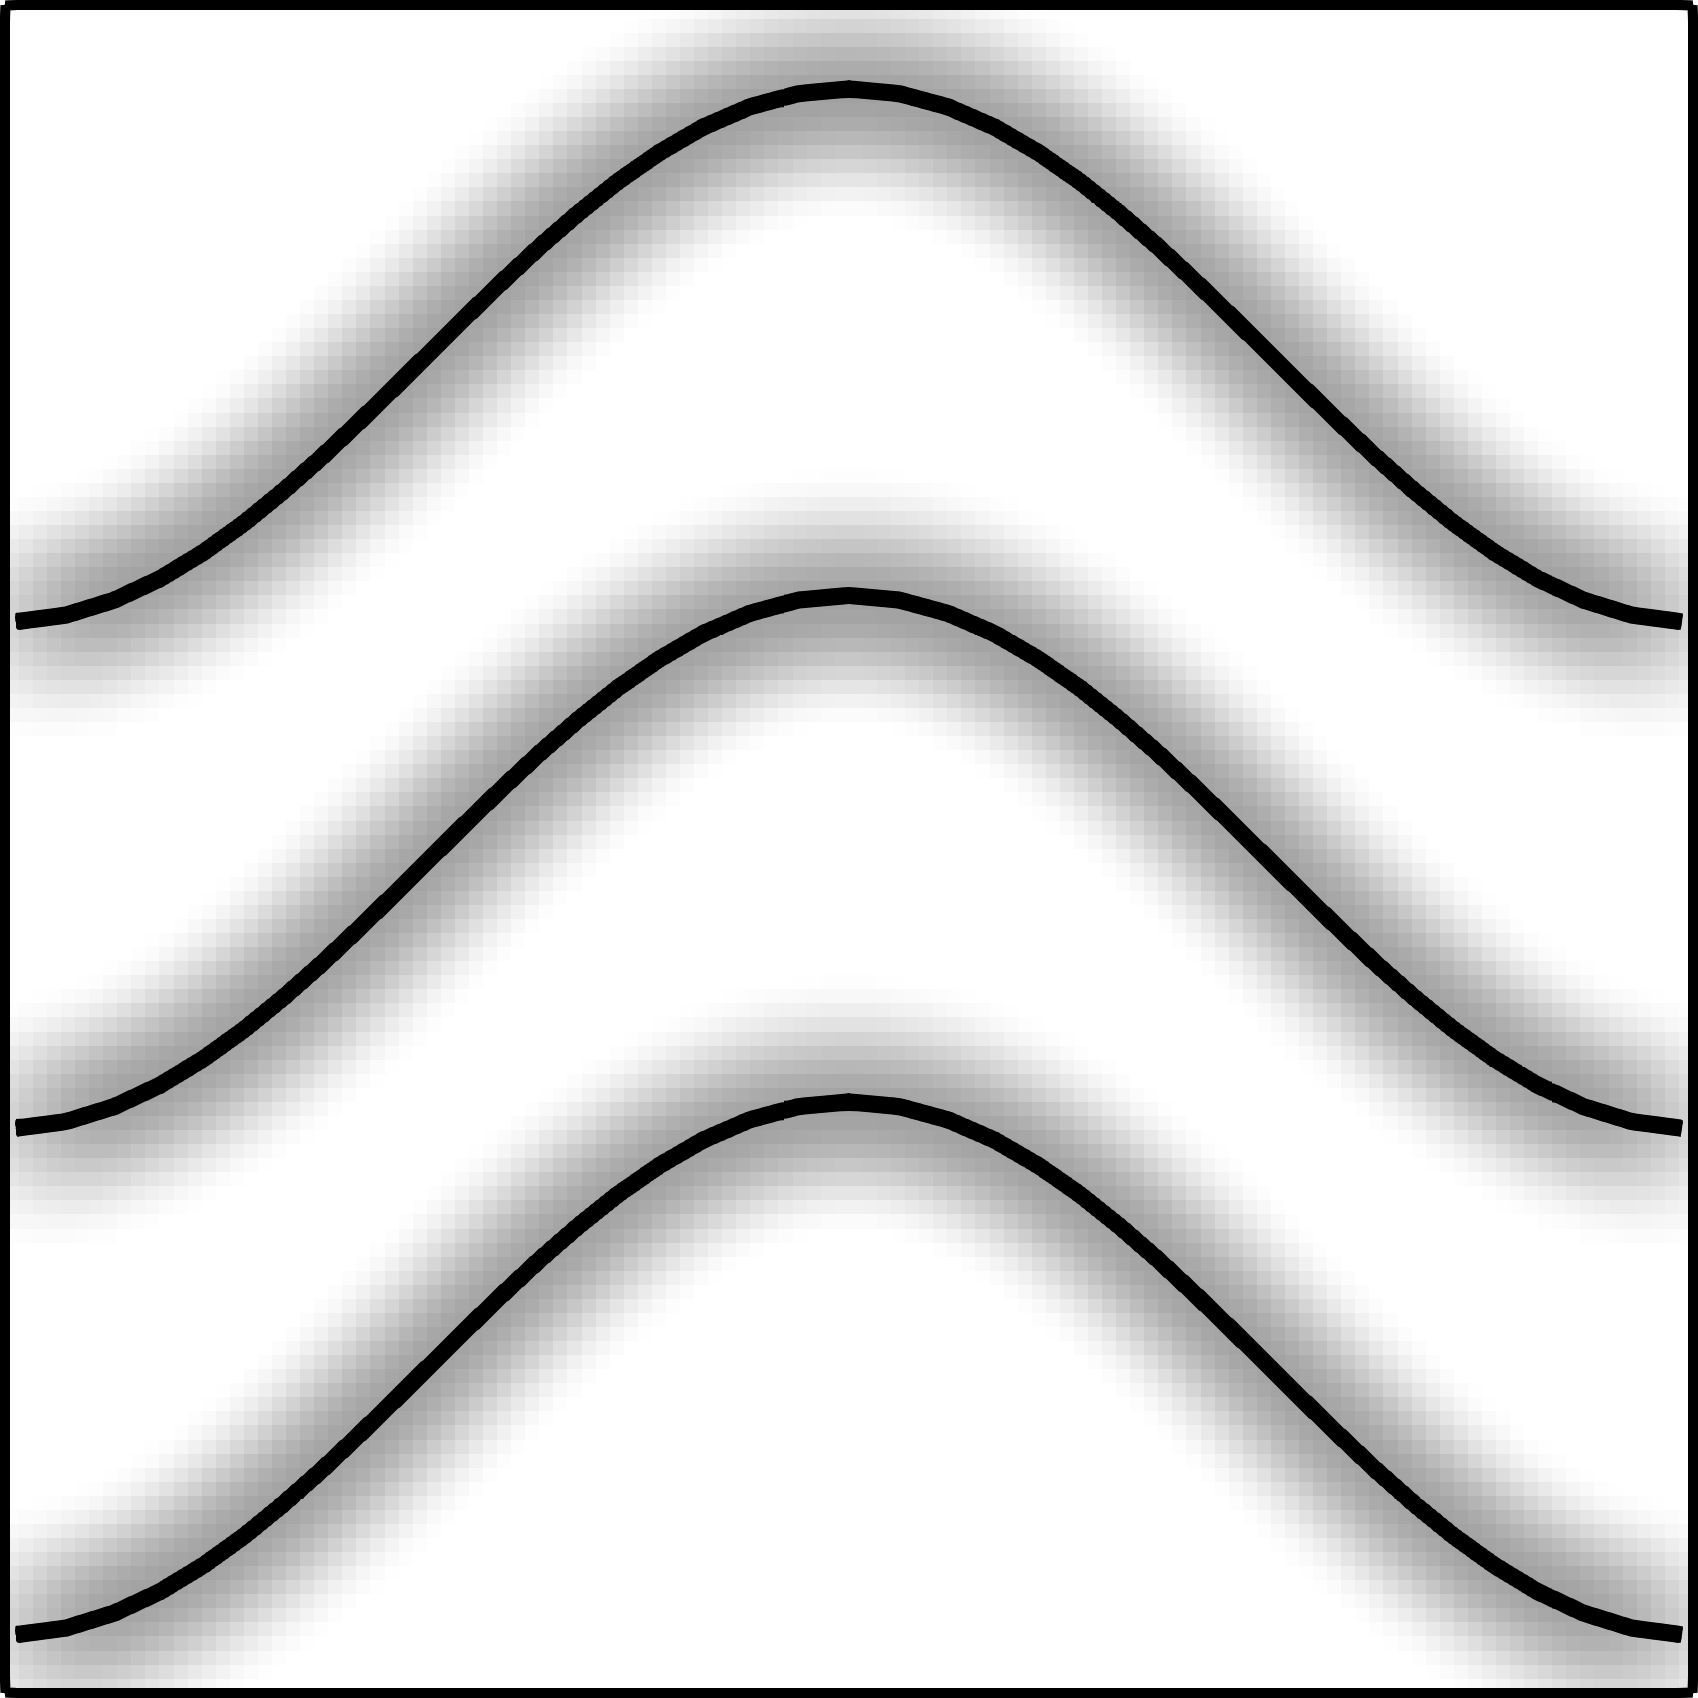
\includegraphics[scale=.08]{figures/Shatter/3Lines.png}
        \caption{}
    \end{subfigure}
    \begin{subfigure}[b]{.3\textwidth}
        \centering
        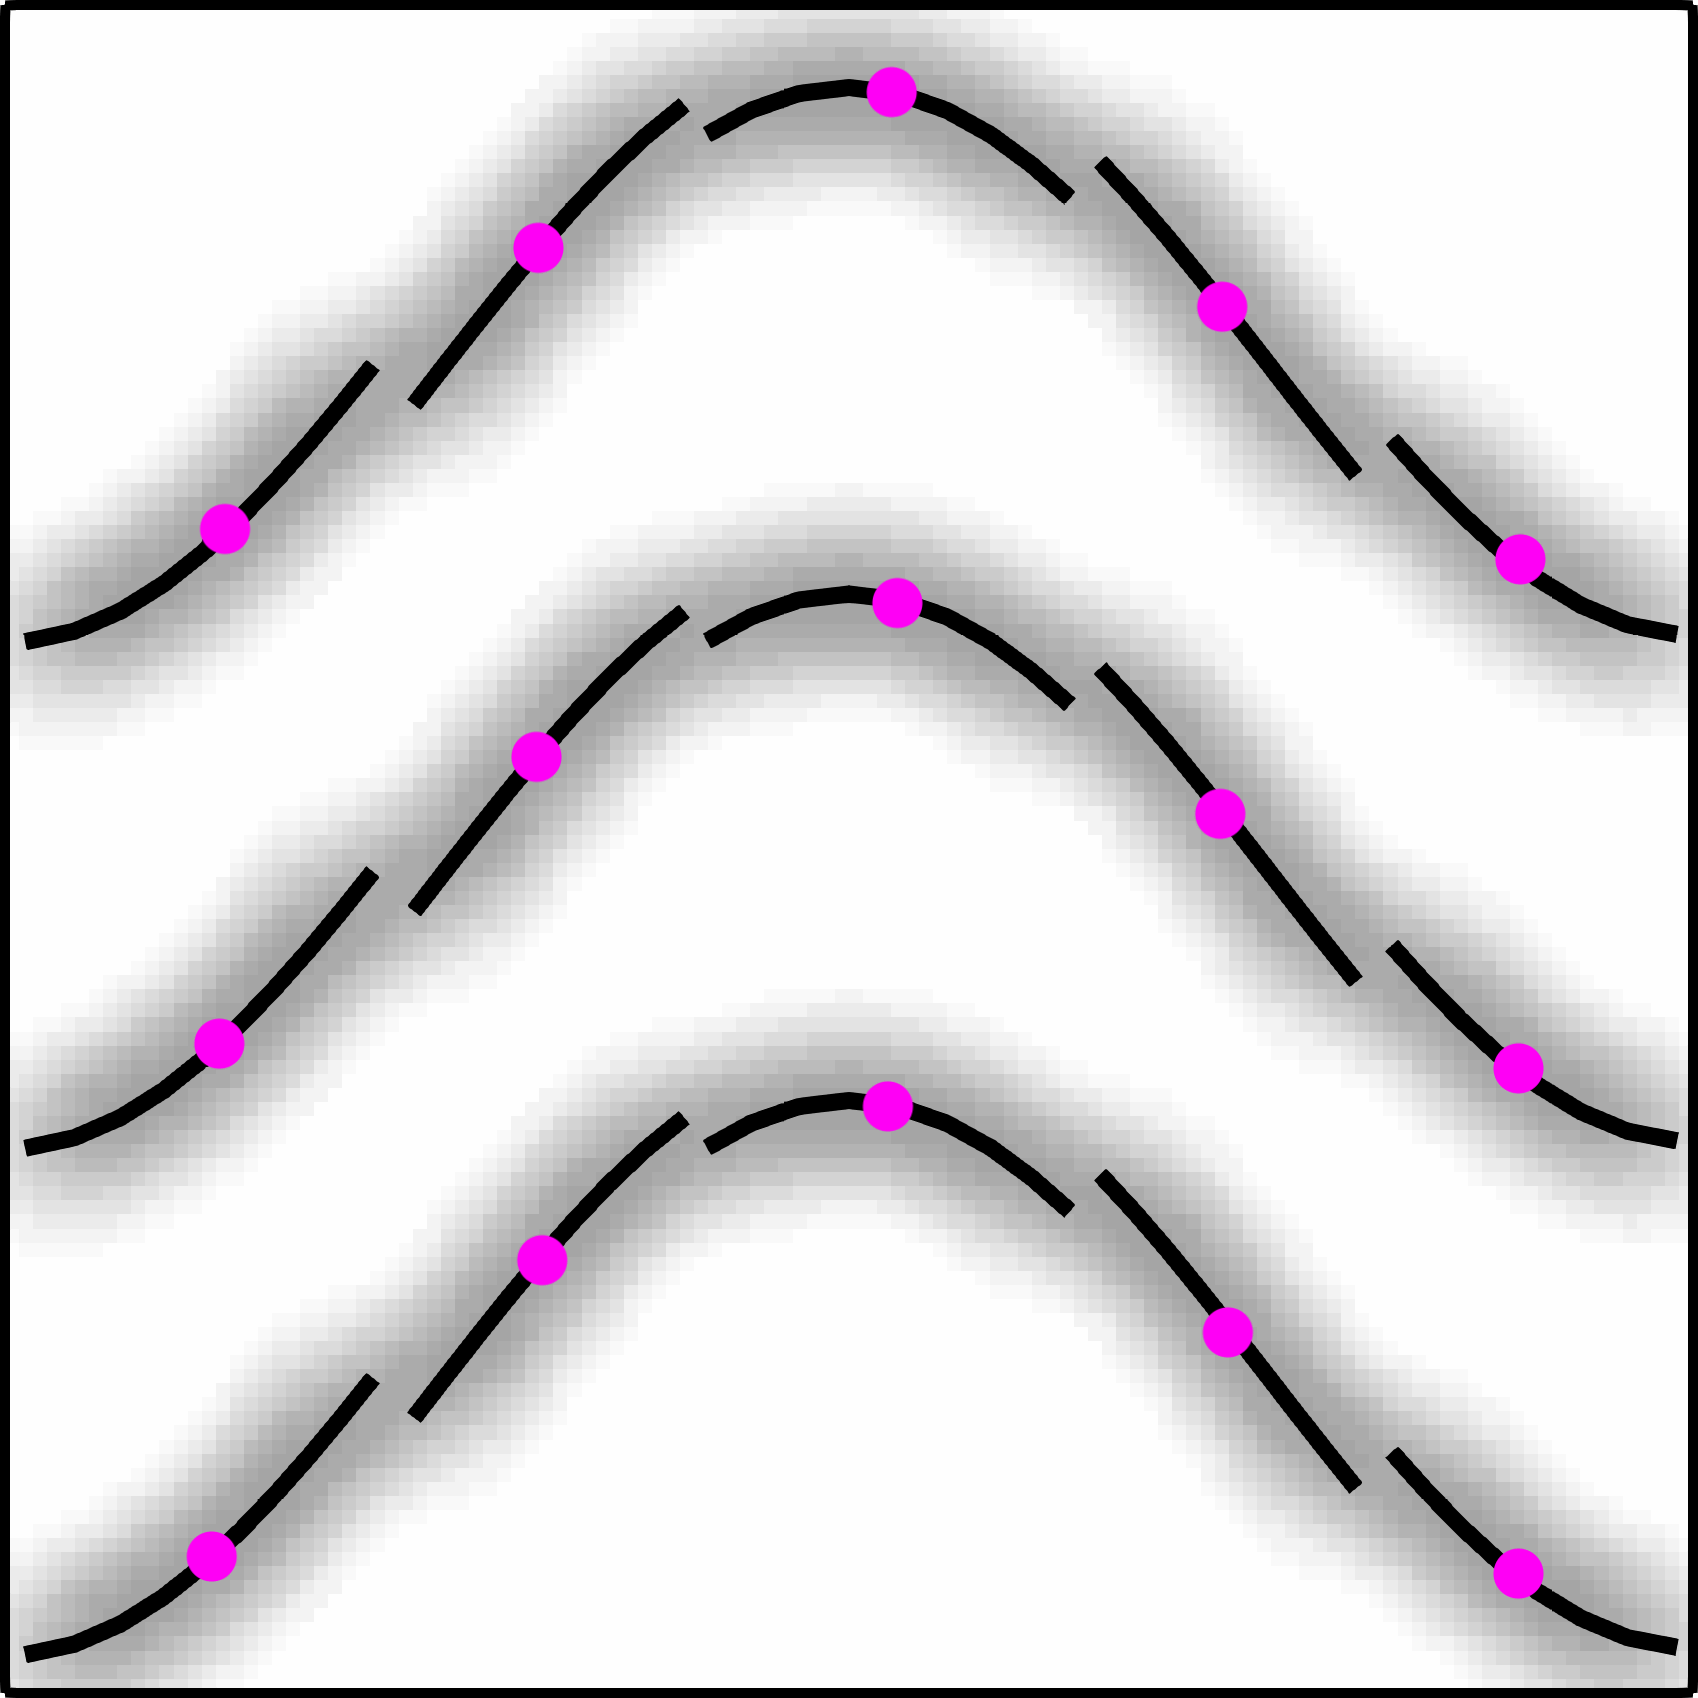
\includegraphics[scale=.08]{figures/Shatter/15Lines.png}
        \caption{}
    \end{subfigure}
    \begin{subfigure}[b]{.3\textwidth}
        \centering
        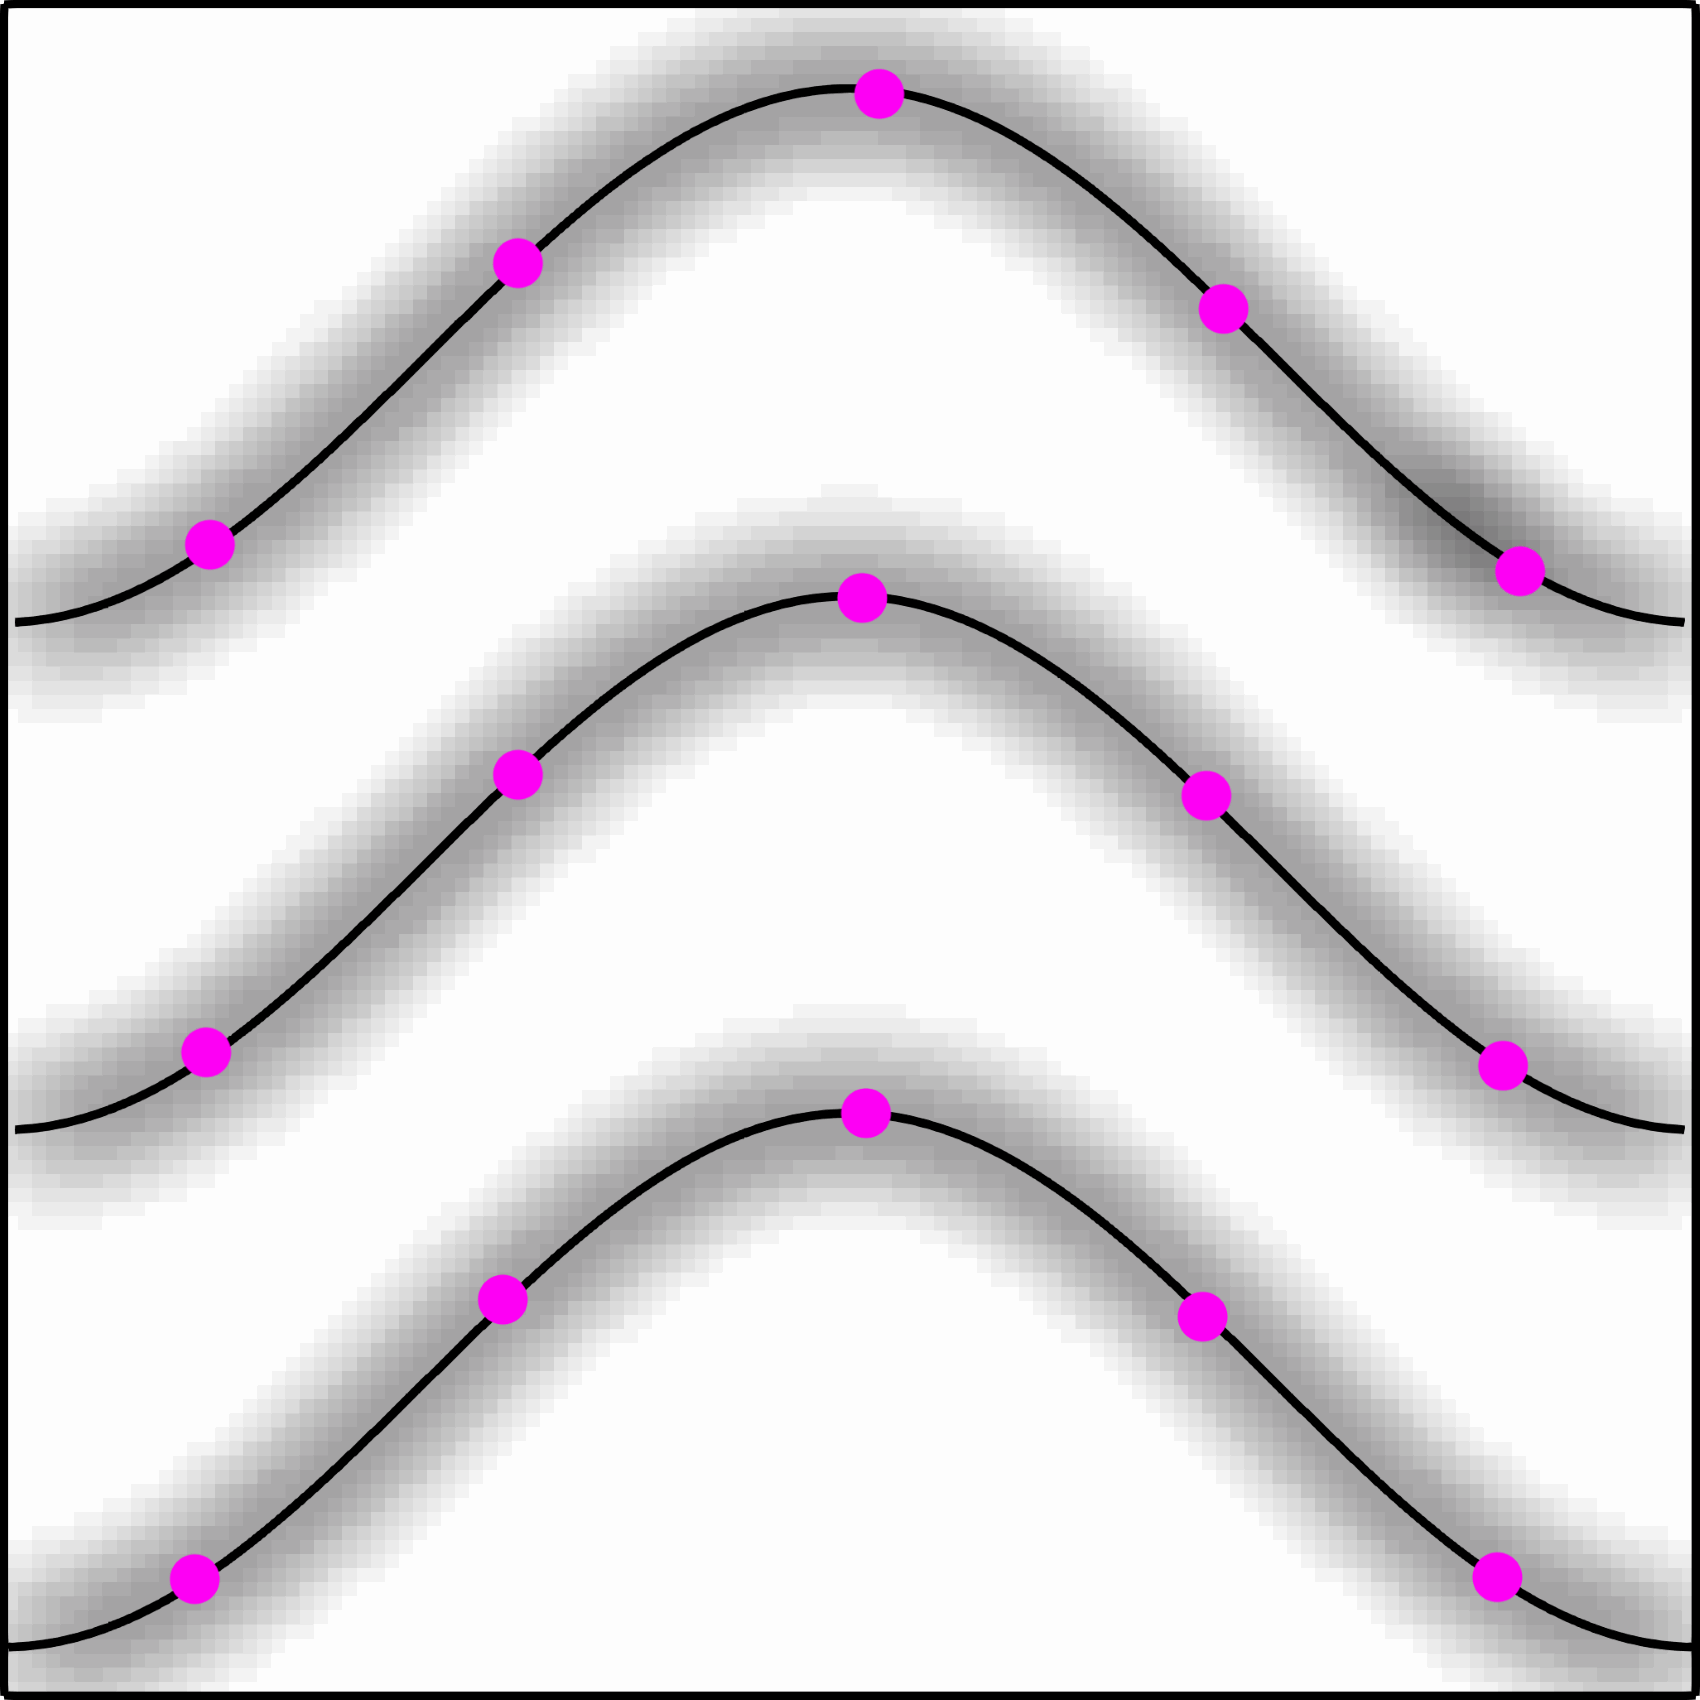
\includegraphics[scale=.08]{figures/Shatter/3LinesRejoin.png}
        \caption{}
    \end{subfigure}
    \caption{
        (a) Three streamlines after being optimized.
        (b) To make the individual shards visible, we change the field's amplitude slightly.
        The shards' seeds are the center of the streamlines in (b), and all lie on one of the streamlines in (a).
        (c) Shards quickly rejoin when redrawn in the same field they originate from (a).
        We used a slightly reduced thickness to make it more visible that the shards
        do not simply overlap but actually rejoin into their single former streamline.
    }
    \label[figure]{fig:rejoin}
\end{figure}


\subsection{Shattering}
At the end of a time step's optimization phase, we break every streamline apart into smaller streamlets we refer to as \textit{shards}.
We start by dividing the parent streamline length-wise into sections which equal the length of the starting streamlines.
The shards are assigned a seed in the middle (lengthwise) of these intervals,
and their length equals the streamline start length.
If the parent streamline has some length remaining because it was not perfectly divisible by the start length, the last shard's length will be shorter.
This leaves each former streamline with the appearance of being dashed with each fragment having its own seed, and can be seen in \cref{fig:rejoin} (b).
The shards then act as the initial seeding strategy for the subsequent timeframe; the regular grid is only used for the first frame.
This way, we obtain many seeds that, if the field does not change too much, will merge back into the streamline they came from, as can be seen in \cref{fig:rejoin} (a) and (c),
saving iterations that would be needed for new seeding and lengthening in these regions.
If the field \textit{does} change, some segments will still reconnect and therefore keep their temporal coherence,
whereas areas of strong fluctuation will connect to different streamlines.
This results in changes being limited to parts where a streamline change is necessary,
providing extra streamlines in these areas while not affecting streamline trajectory too much on a global level.
\newpage

% \begin{figure}[ht]
%     \centering
%     \begin{subfigure}[b]{.32\textwidth}
%         \centering
%         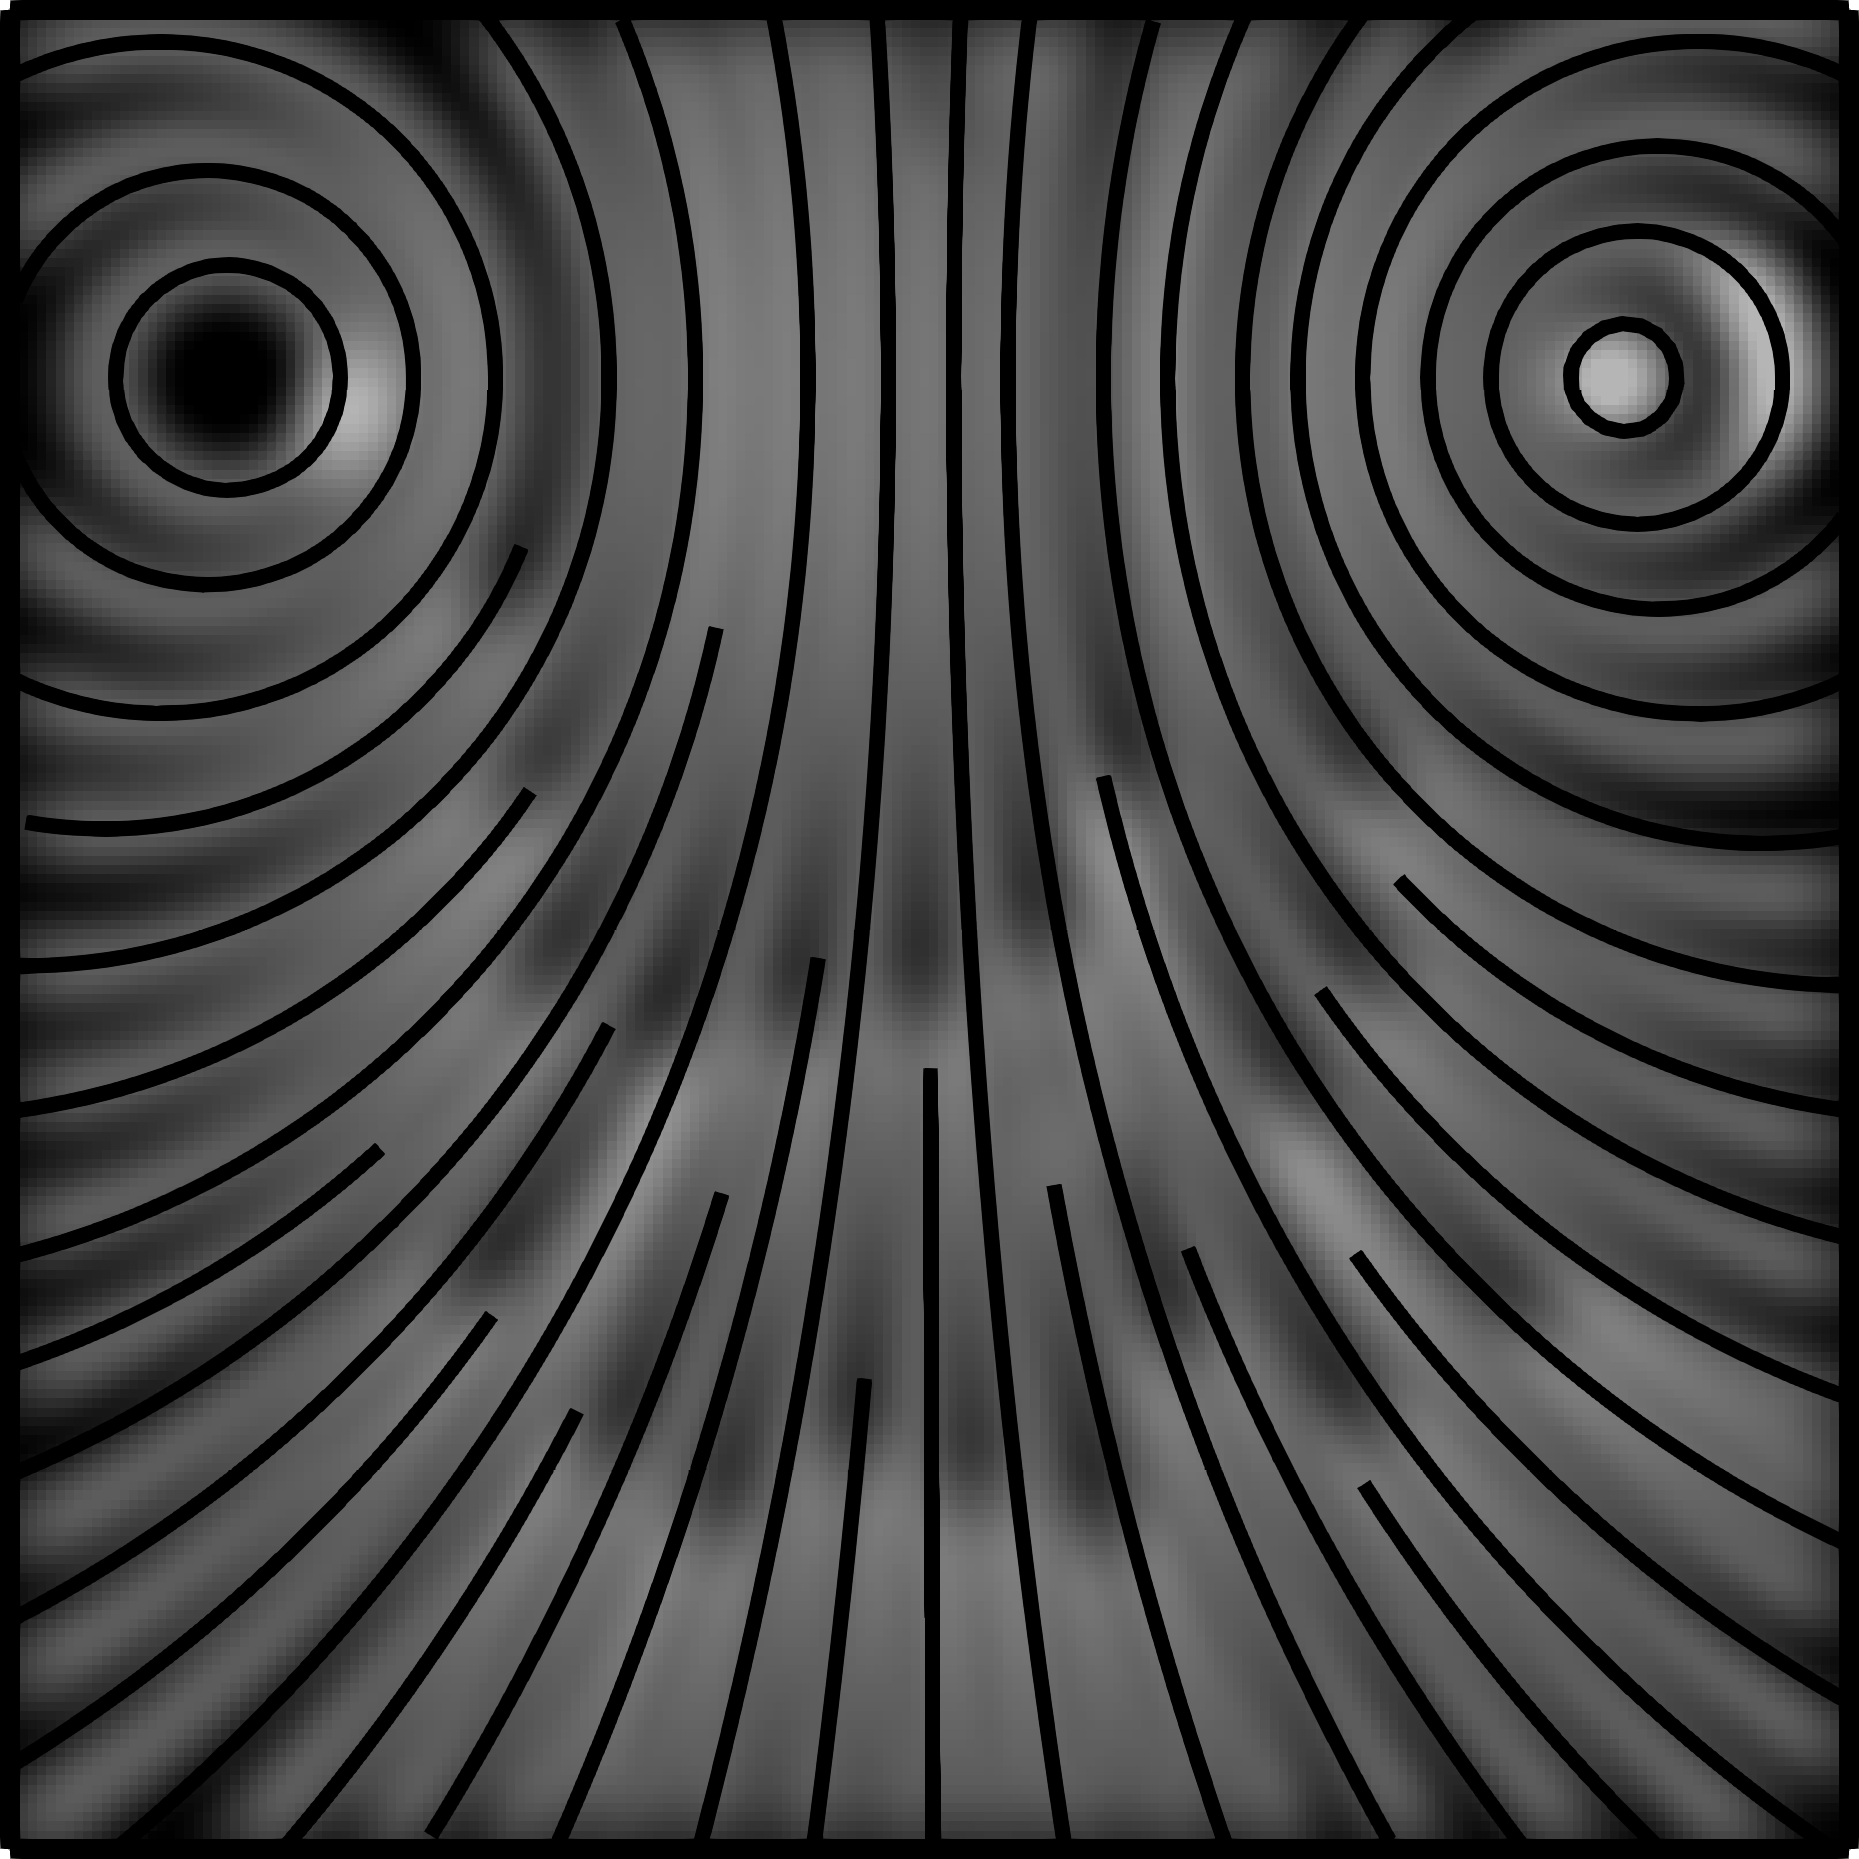
\includegraphics[scale=.08]{figures/TBGyro.png}
%         \caption{}
%     \end{subfigure}
%     \begin{subfigure}[b]{.32\textwidth}
%         \centering
%         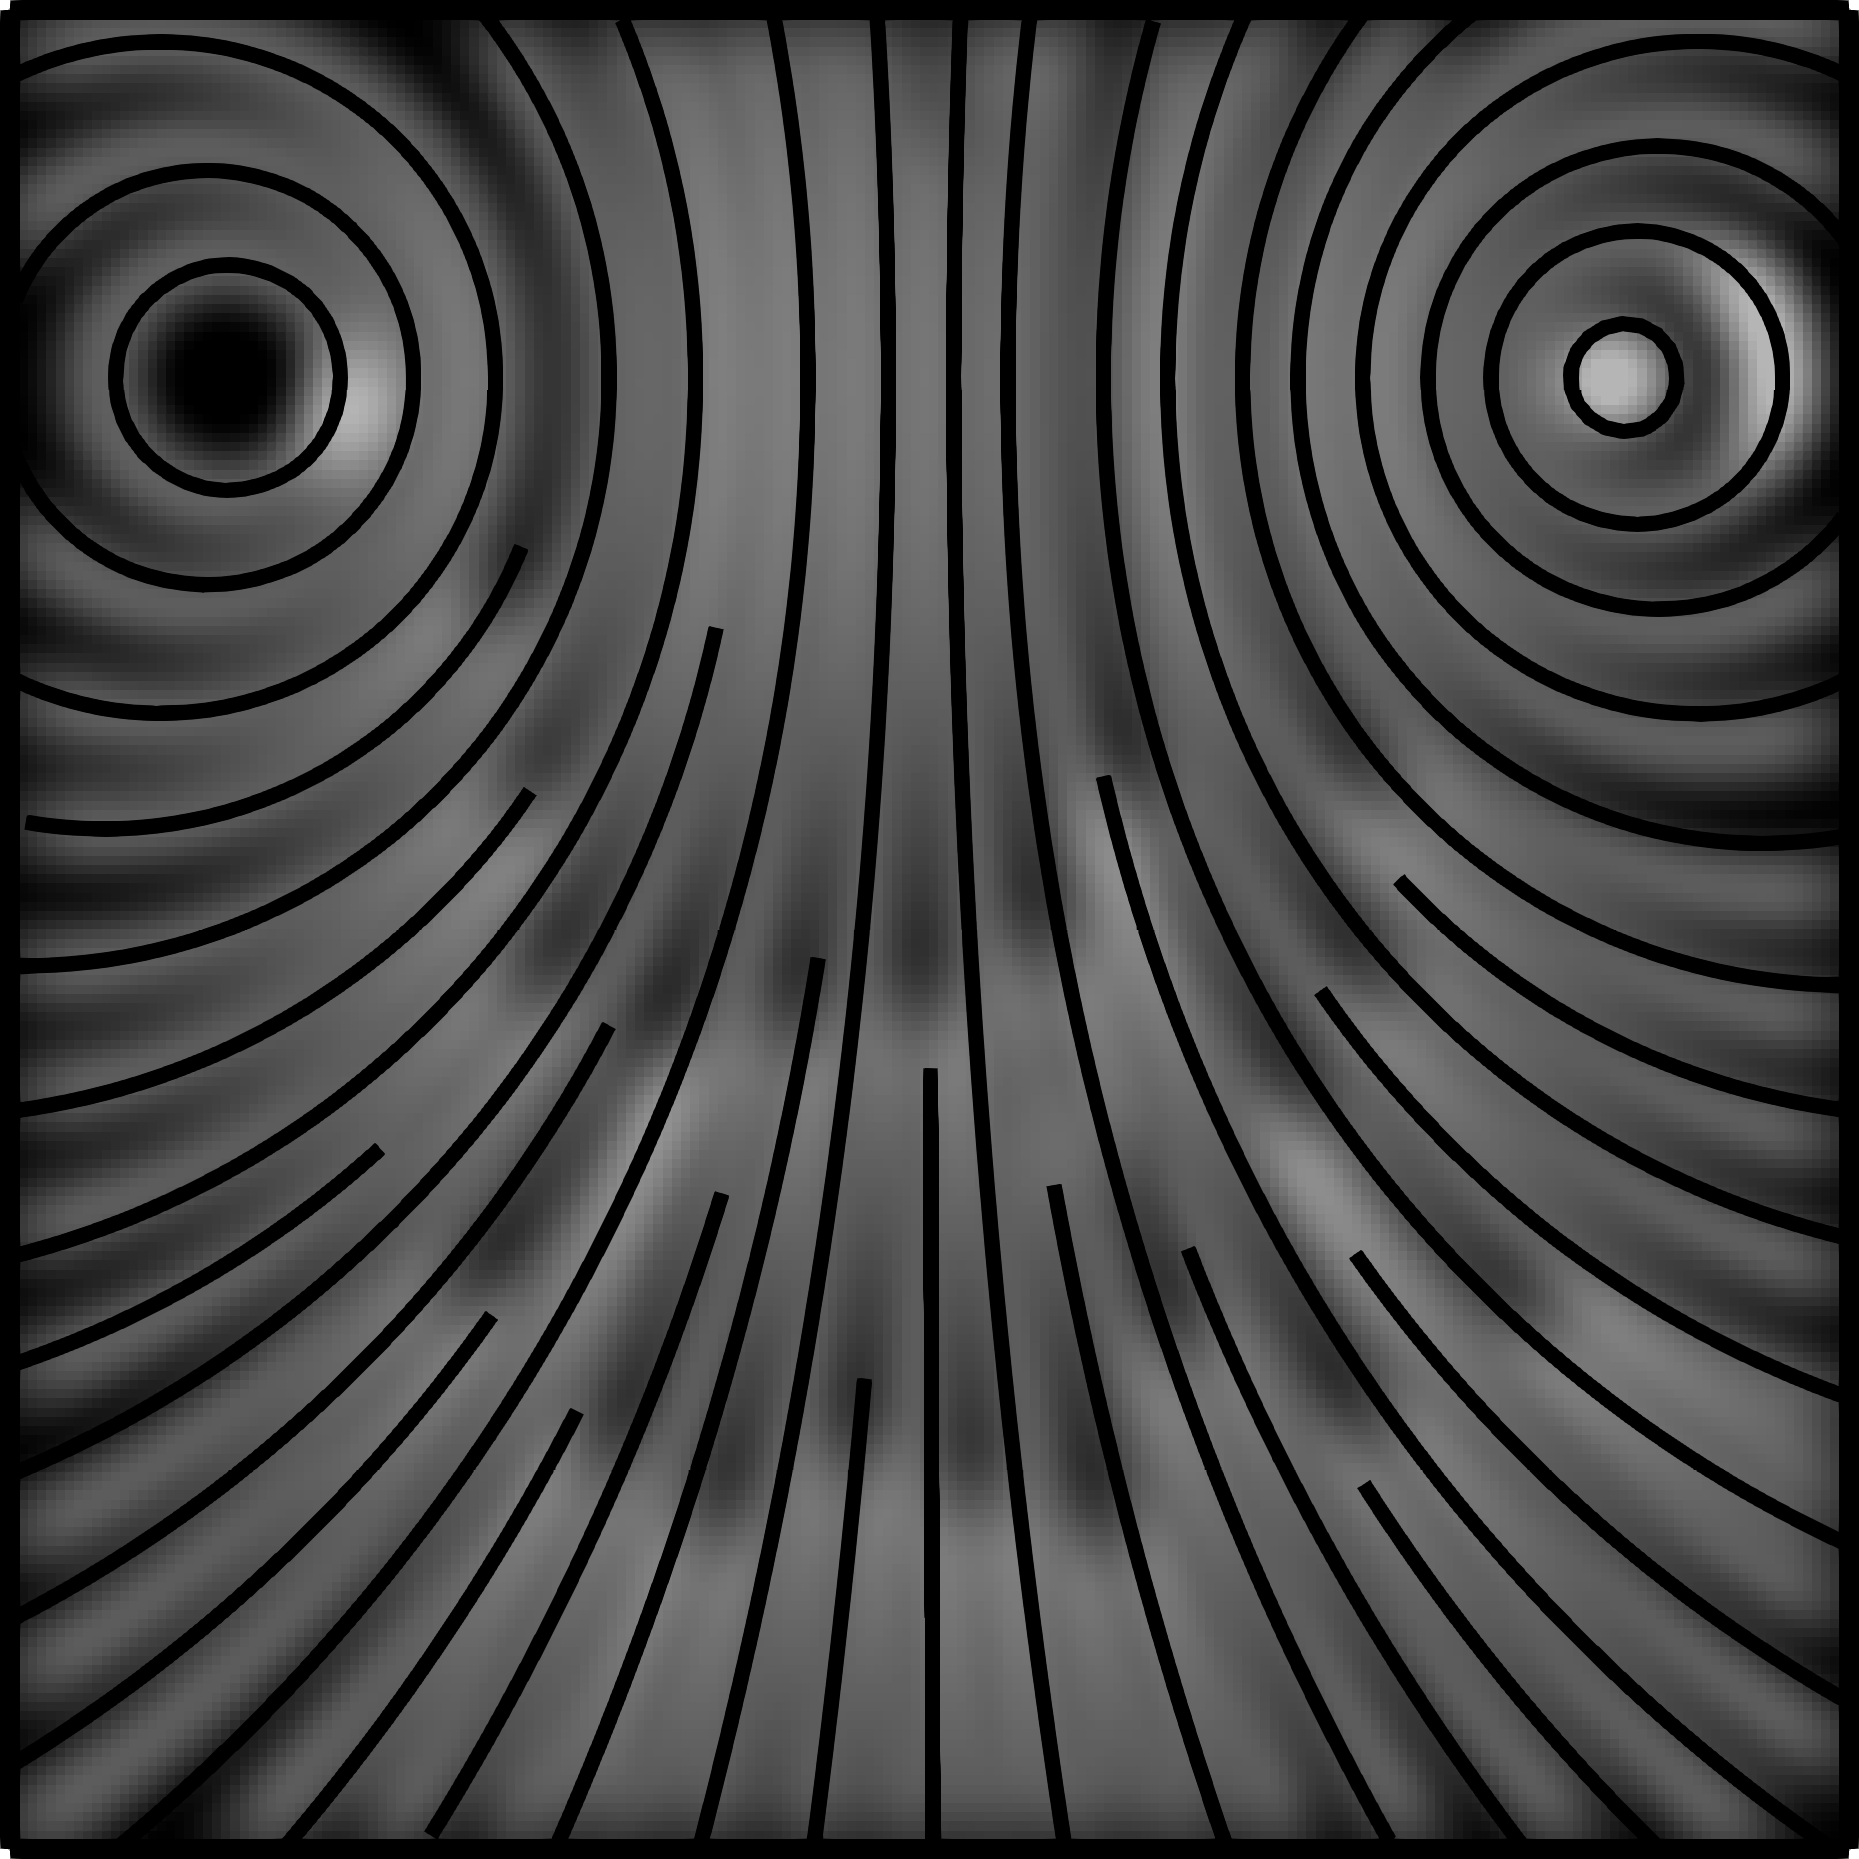
\includegraphics[scale=.08]{figures/TBGyro.png}
%         \caption{}
%     \end{subfigure}
%     \begin{subfigure}[b]{.32\textwidth}
%         \centering
%         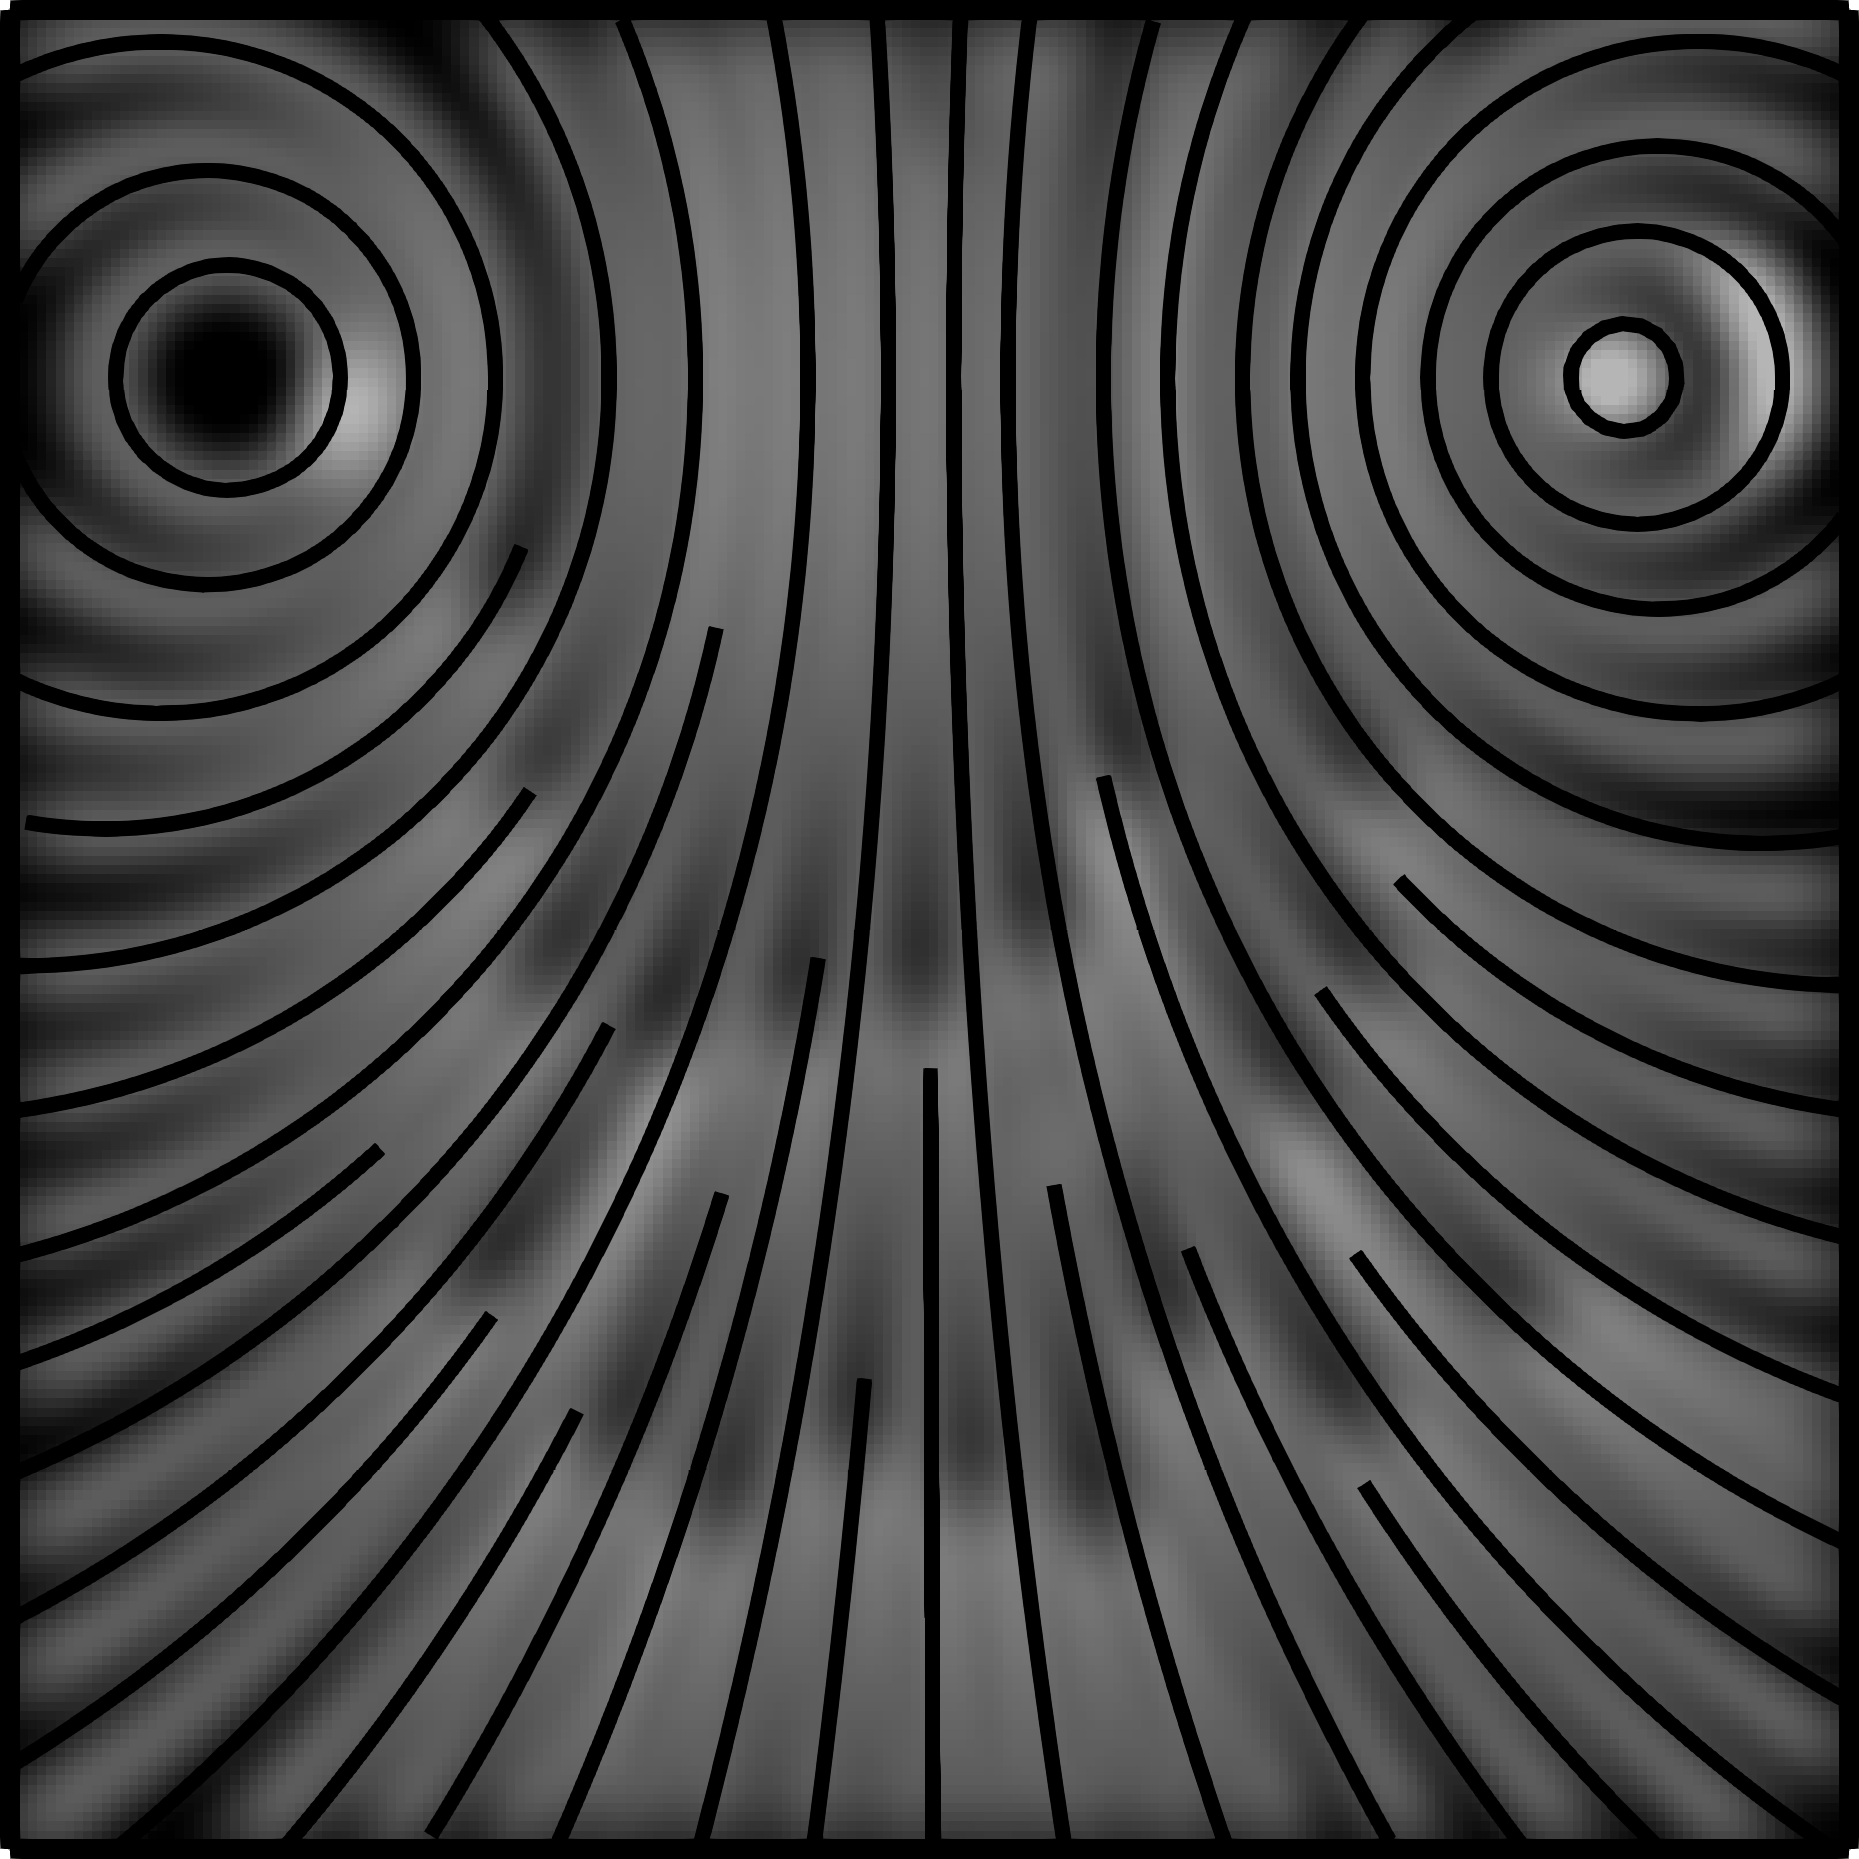
\includegraphics[scale=.08]{figures/TBGyro.png}
%         \caption{}
%     \end{subfigure}
%     \caption{
%         (a): Two time steps without shattering.
%         (b): Two time steps with shattering.
%         (c): Total energy vs iteration step for (a) and (b).
%     }
%     \label[figure]{fig:combined}
% \end{figure}

\subsection{Combining Shattering and Coaxing}
Combining shattering and coaxing, we obtain a more reliable way of generating streamlines according to the footprint left behind by the last frame.
The seeds created during the shatter process all lie inside the footprint left behind by the previous streamline path.
Due to the coaxing function of the modified energy measure, it is unlikely that they will leave this valley solely due to the random movements of relaxation.
A change in the field is necessary in order to overcome the weight of the time coherence, making the streamline move or grow outside the previous footprint.
Due to the seeds being held in place in this way, it is very likely for them to rejoin to form the same lane they originated from.
If the field changes drastically in this region, the seeds can not fully connect to each other anymore, and will instead gravitate to a different footprint,
forming long patches of coherent streamlines whenever possible while still allowing relaxation to ensure good spatial distribution.\\
% In \cref{fig:combined} (c),
% we see that joining shards to form the streamlines is significantly faster than generating them anew.


